%%%%%%%%%%%%%%%%%%%%%%%%%%%%%%%%%%%%%%%%%%%%%%%%%%%%%%%%%%%%%%%%%%%%%%
% Overleaf (WriteLaTeX) Example: Molecular Chemistry Presentation
%
% Source: http://www.overleaf.com
%
% In these slides we show how Overleaf can be used with standard 
% chemistry packages to easily create professional presentations.
% 
% Feel free to distribute this example, but please keep the referral
% to overleaf.com
% 
%%%%%%%%%%%%%%%%%%%%%%%%%%%%%%%%%%%%%%%%%%%%%%%%%%%%%%%%%%%%%%%%%%%%%%

\documentclass{beamer}

\mode<presentation>
{
  \usetheme{Madrid}       % or try default, Darmstadt, Warsaw, ...
  \usecolortheme{default} % or try albatross, beaver, crane, ...
  \usefonttheme{default}    % or try default, structurebold, ...
  \setbeamertemplate{navigation symbols}{}
  \setbeamertemplate{caption}[numbered]
} 

\usepackage[english]{babel}
\usepackage[utf8x]{inputenc}
\usepackage{chemfig}
\usepackage[version=3]{mhchem}

\usepackage{hyperref}
  \hypersetup{colorlinks=true}
  \hypersetup{urlcolor=blue}
  \hypersetup{linkcolor = .}
\usepackage{xcolor}
\usepackage{siunitx}
  \sisetup{separate-uncertainty = true}
\usepackage{physics}
\usepackage[font=small,labelfont=bf]{caption}
\usepackage{subcaption}
\usepackage[en-GB]{datetime2}
\usepackage{overpic}
\usepackage{feynmp}
\DeclareGraphicsRule{*}{mps}{*}{}

\usepackage{scalerel}
\newcommand{\mylbrace}[2]{\vspace{#2pt}\hspace{6pt}\scaleleftright[\dimexpr5pt+#1\dimexpr0.06pt]{\lbrace}{\rule[\dimexpr2pt-#1\dimexpr0.5pt]{-4pt}{#1pt}}{.}}
\newcommand{\myrbrace}[2]{\vspace{#2pt}\scaleleftright[\dimexpr5pt+#1\dimexpr0.06pt]{.}{\rule[\dimexpr2pt-#1\dimexpr0.5pt]{-4pt}{#1pt}}{\rbrace}\hspace{6pt}}

% Here's where the presentation starts, with the info for the title slide
\title[University of Oxford]{BESIII Charm Meeting \\Measurement of CP even fraction $F_+$ in $D^0\to K^+K^-\pi^+\pi^-$}
%\author{\textbf{Martin Tat} \hspace{0.54em} Guy Wilkinson \hspace{0.54em} Sneha Malde}
\author{Martin Tat}
\institute{University of Oxford}
\date{15th March 2022}

\titlegraphic{
\includegraphics[width = 2.0cm, height = 2.0cm]{OxfordLogo.pdf}\hspace{1cm}~%
              
\includegraphics[width = 3.2cm, height = 2.0cm]{bes3.jpg}}

\begin{document}

\begin{frame}
  \titlepage
\end{frame}

% These three lines create an automatically generated table of contents.
\begin{frame}{Outline}
  \tableofcontents
\end{frame}

\section{Introduction and motivation}
\begin{frame}{Introduction}
  \begin{itemize}
    \setlength\itemsep{0.5em}
    \item{Original plan (for my PhD):}
    \begin{itemize}
    \setlength\itemsep{0.2em}
      \item{$c_i$/$s_i$ analysis with new $\SI{20}{\per\femto\barn}$ BESIII $\psi(3770)$ dataset}
      \item{Develop binning scheme using LHCb model \href{https://arxiv.org/abs/1811.08304}{JHEP 02 (2019) 126}}
      \item{Perform model independent $\gamma$ measurement at LHCb simultaneously}
      \begin{itemize}
        \item{Expected precision $\Delta\gamma\approx 12^\circ$ with LHCb Run\,1+2}
      \end{itemize}
    \end{itemize}
  \end{itemize}
  \begin{figure}
    \centering
    \begin{subfigure}{0.5\textwidth}
      \centering
      \begin{overpic}[width=1.0\textwidth, clip=true, trim={10.0cm 2.7cm 0.8cm 0}]{Plots/d2kkpipi_fiveL_allDP.pdf}
        \put (55,58) {\scriptsize LHCb unofficial}
      \end{overpic}
      \caption{Fit of $B^\pm\to[K^+K^-\pi^+\pi^-]_D\pi^\pm$}
    \end{subfigure}%
    \begin{subfigure}{0.5\textwidth}
      \centering
      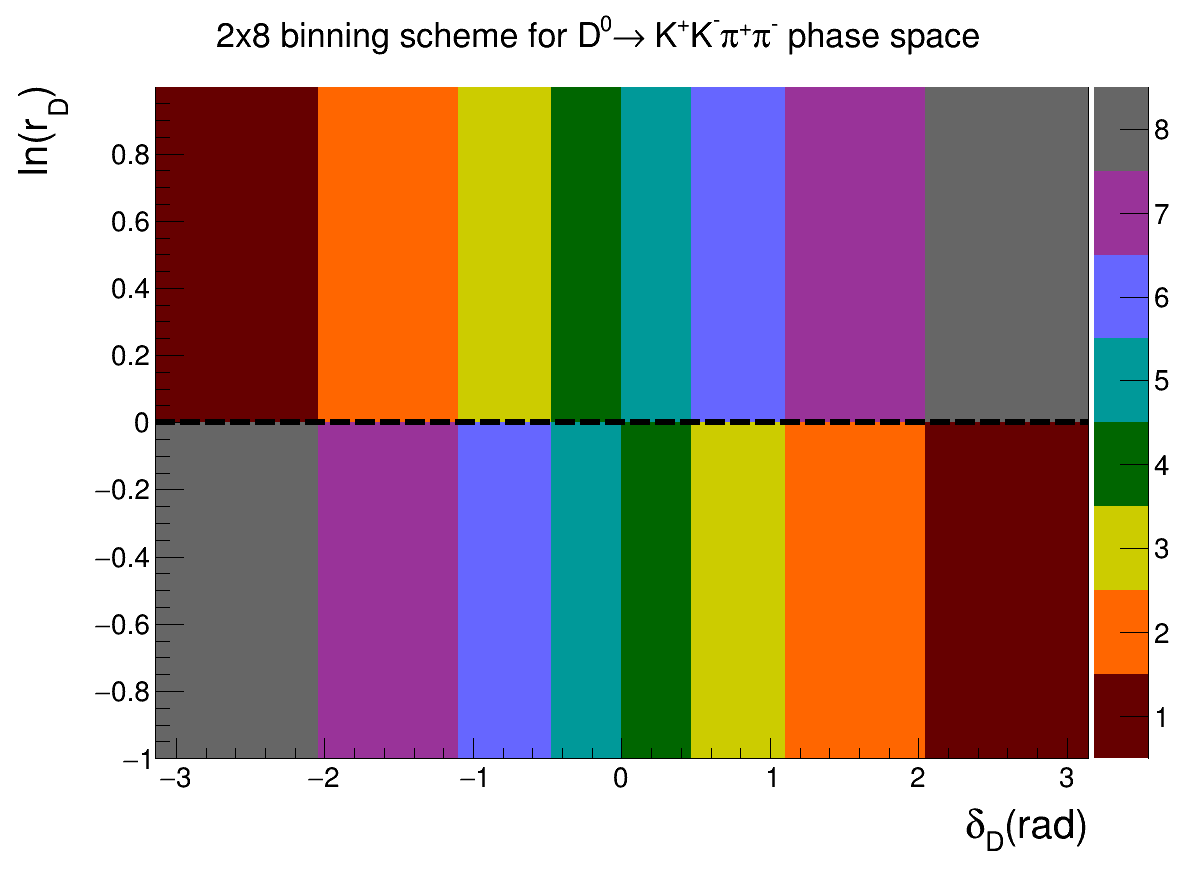
\includegraphics[width=\textwidth]{Plots/BinningSchemePlot_8Bins.png}
      \caption{Binning scheme for $D^0\to K^+K^-\pi^+\pi^-$}
    \end{subfigure}
  \end{figure}
\end{frame}

\begin{frame}{Motivation}
  \begin{itemize}
    \setlength\itemsep{1.0em}
    \item{$F_+$ describes the CP content of a self-conjugate multi-body decay}
    \begin{itemize}
      \item{$F_+ = 1$ ($0$) for CP even (odd) final states}
    \end{itemize}
    \item{$F_+$ can be measured with current $\SI{3}{\per\femto\barn}$ dataset}
    \begin{itemize}
      \item{First model independent measurement of $F_+^{KK\pi\pi}$!}
      \item{Useful to test agreement with LHCb model prediction: $F_+ = 0.73$}
    \end{itemize}
    \item{Important input to quasi-GLW analysis of the CKM angle $\gamma$}
    \begin{itemize}
      \item{Current GLW modes: $KK$, $\pi\pi$, $\pi\pi\pi\pi$}
      \item{Minimal effort to include $KK\pi\pi$ in GLW analyses $\implies$ More statistics}
    \end{itemize}
    \item{Other $F_+$ measurements:}
    \begin{itemize}
      \item{$D^0\to\pi^+\pi^-\pi^+\pi^-$ \href{https://arxiv.org/abs/1709.03467}{JHEP 01 (2018) 144}}
      \item{$D^0\to K_S\pi^+\pi^-\pi^0$ \href{https://arxiv.org/abs/1710.10086}{JHEP 01 (2018) 82}}
      \item{Both measurements are from CLEO-c, BESIII analyses ongoing}
    \end{itemize}
  \end{itemize}
\end{frame}

\section{Strategy of strong-phase analysis}
\begin{frame}{Strategy for strong-phase analysis}
  \begin{enumerate}
    \setlength\itemsep{0.5em}
    \item{Select double tags of $KK\pi\pi$ vs flavour, CP and self-conjugate tags}
    \item{Measure flavour tag yields $K_i$}
    \item{Measure $c_i$ with CP tags:}
    \item{Measure $c_i$+$s_i$ with self-conjugate tags}
  \end{enumerate}
  \begin{block}{$c_i$/$s_i$ analysis}
    CP: $M_i\propto\big(K_i + K_{-i} - 2c_i\sqrt{K_iK_{-i}}(2F_+^{\rm tag} - 1)\big)$ \\
    Self-conjugate: $M_{ij}\propto\big(K_iK_{-j}^\prime + K_{-i}K_j^\prime - 2\sqrt{K_iK_{-i}K_j^\prime K_{-j}^\prime}(c_ic_j^\prime + s_is_{-j}^\prime\big)$
  \end{block}
  \begin{itemize}
    \item{Sum over all $KK\pi\pi$ bins to measure $F_+^{KK\pi\pi}$:}
  \end{itemize}
  \begin{block}{$F_+$ analysis}
    CP: $M\propto\big(1 - 2(2F_+^{KK\pi\pi} - 1)(2F_+^{\rm tag} - 1)\big)$ \\
    Self-conjugate: $M_j\propto\big(K_j^\prime + K_{-j}^\prime - 2c_j^{\prime}\sqrt{K_j^\prime K_{-j}^\prime}(2F_+^{KK\pi\pi} - 1)\big)$
  \end{block}
\end{frame}

\section{Selection and tag modes}
\begin{frame}{Selection}
  \begin{itemize}
    \item{Selection of charged and neutral particles follow standard track and shower requirements}
    \item{Require flight significance $> 2$ for $K_S$}
    \item{$K_S$ veto for $KK\pi\pi$ and $\pi\pi\pi^0$ tags}
    \item{$\Delta E$ cut of $3\sigma$}
    \item{$\Delta E$ fit for 4-body modes allow a non-smooth background at $\Delta E = 0$}
  \end{itemize}
  \begin{figure}
    \centering
    \begin{subfigure}{0.5\textwidth}
      \centering
      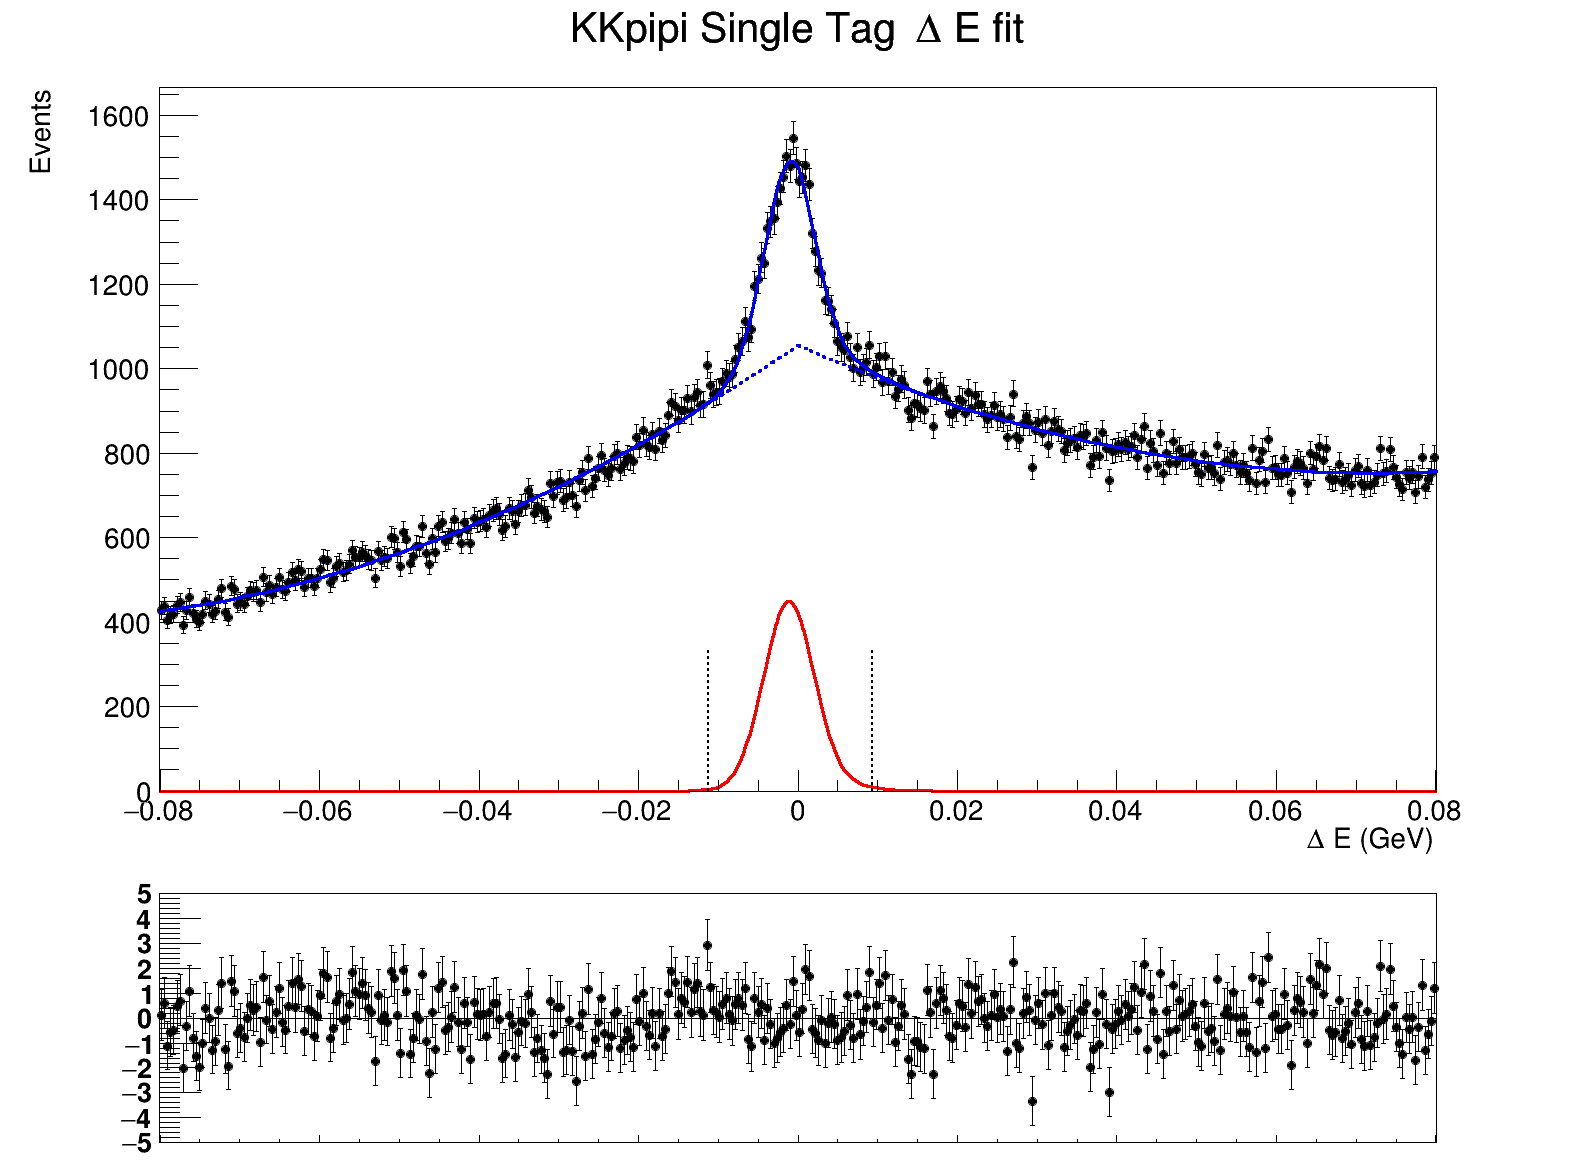
\includegraphics[width=\textwidth, clip = true, trim = {0 11cm 0 0 }]{Plots/KKpipi_SingleTag_DeltaE_Plot.png}
    \end{subfigure}%
    \begin{subfigure}{0.5\textwidth}
      \centering
      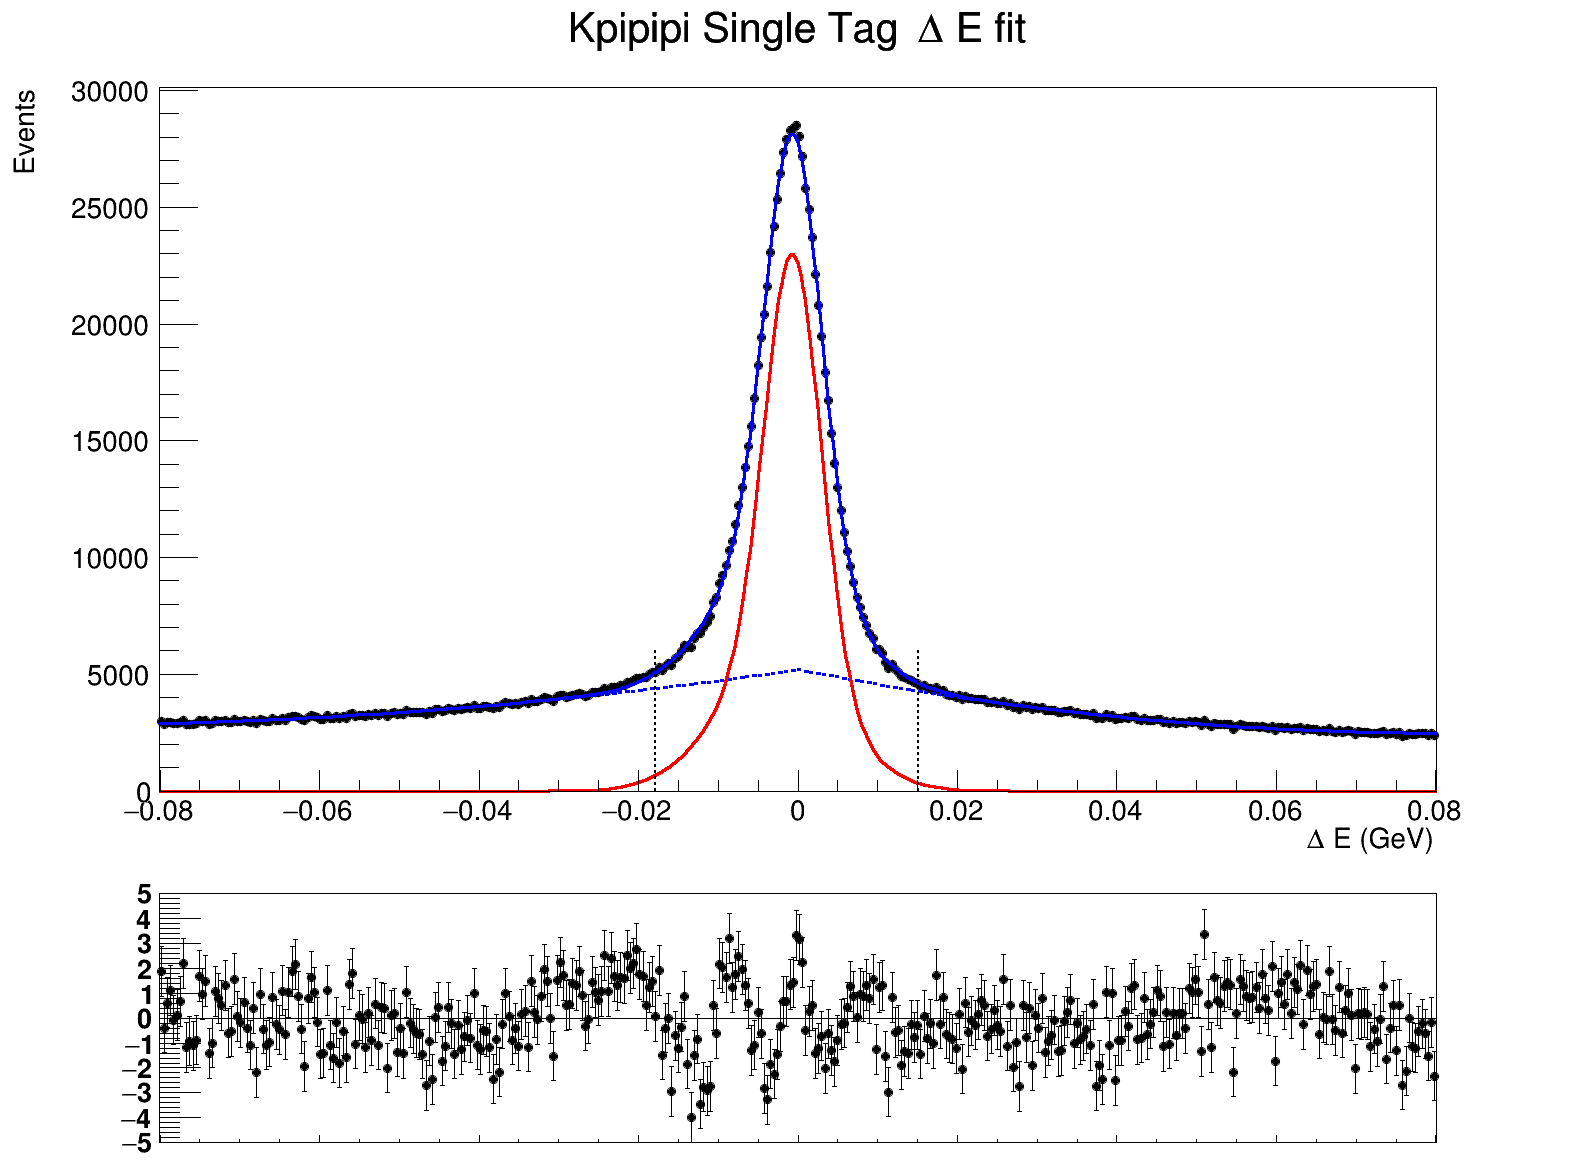
\includegraphics[width=\textwidth, clip = true, trim = {0 11cm 0 0 }]{Plots/Kpipipi_SingleTag_DeltaE_Plot.png}
    \end{subfigure}
    \caption{Double Gaussian signal and Chebychev polynomial background}
  \end{figure}
\end{frame}

\renewcommand*{\thefootnote}{\fnsymbol{footnote}}
\begin{frame}{Tag modes}
  \begin{itemize}
    \setlength\itemsep{1.0em}
    \item{Flavour tags:}
    \begin{itemize}
      \item{$K\pi$, $K\pi\pi^0$, $K\pi\pi\pi$, \underline{$Ke\nu$}}
    \end{itemize}
    \item{CP even tags:}
    \begin{itemize}
      \item{$KK$, $\pi\pi$, $\pi\pi\pi^0$\footnote{Mostly CP even}, $K_S\pi^0\pi^0$, $K_L\pi^0$, \underline{$K_L\omega$}}
    \end{itemize}
    \item{CP odd tags:}
    \begin{itemize}
      \item{$K_S\pi^0$, $K_S\eta$, $K_S\omega$, $K_S\eta^\prime_{\pi\pi\eta}$, $K_S\eta^\prime_{\rho\gamma}$, \underline{$K_L\pi^0\pi^0$}}
    \end{itemize}
    \item{Self-conjugate tags:}
    \begin{itemize}
      \item{$K_S\pi\pi$, $K_L\pi\pi$}
    \end{itemize}
  \end{itemize}
  Underlined tags have not been finalized yet
\end{frame}

\section{Determination of single and double tag yields}
\begin{frame}{Single tag fits}
  \begin{itemize}
    \item{Fit model:}
    \begin{itemize}
      \item{Signal: PDF from signal MC, convoluted with double Gaussian}
      \item{Combinatorial background: Argus PDF}
    \end{itemize}
  \end{itemize}
  \begin{figure}
    \centering
    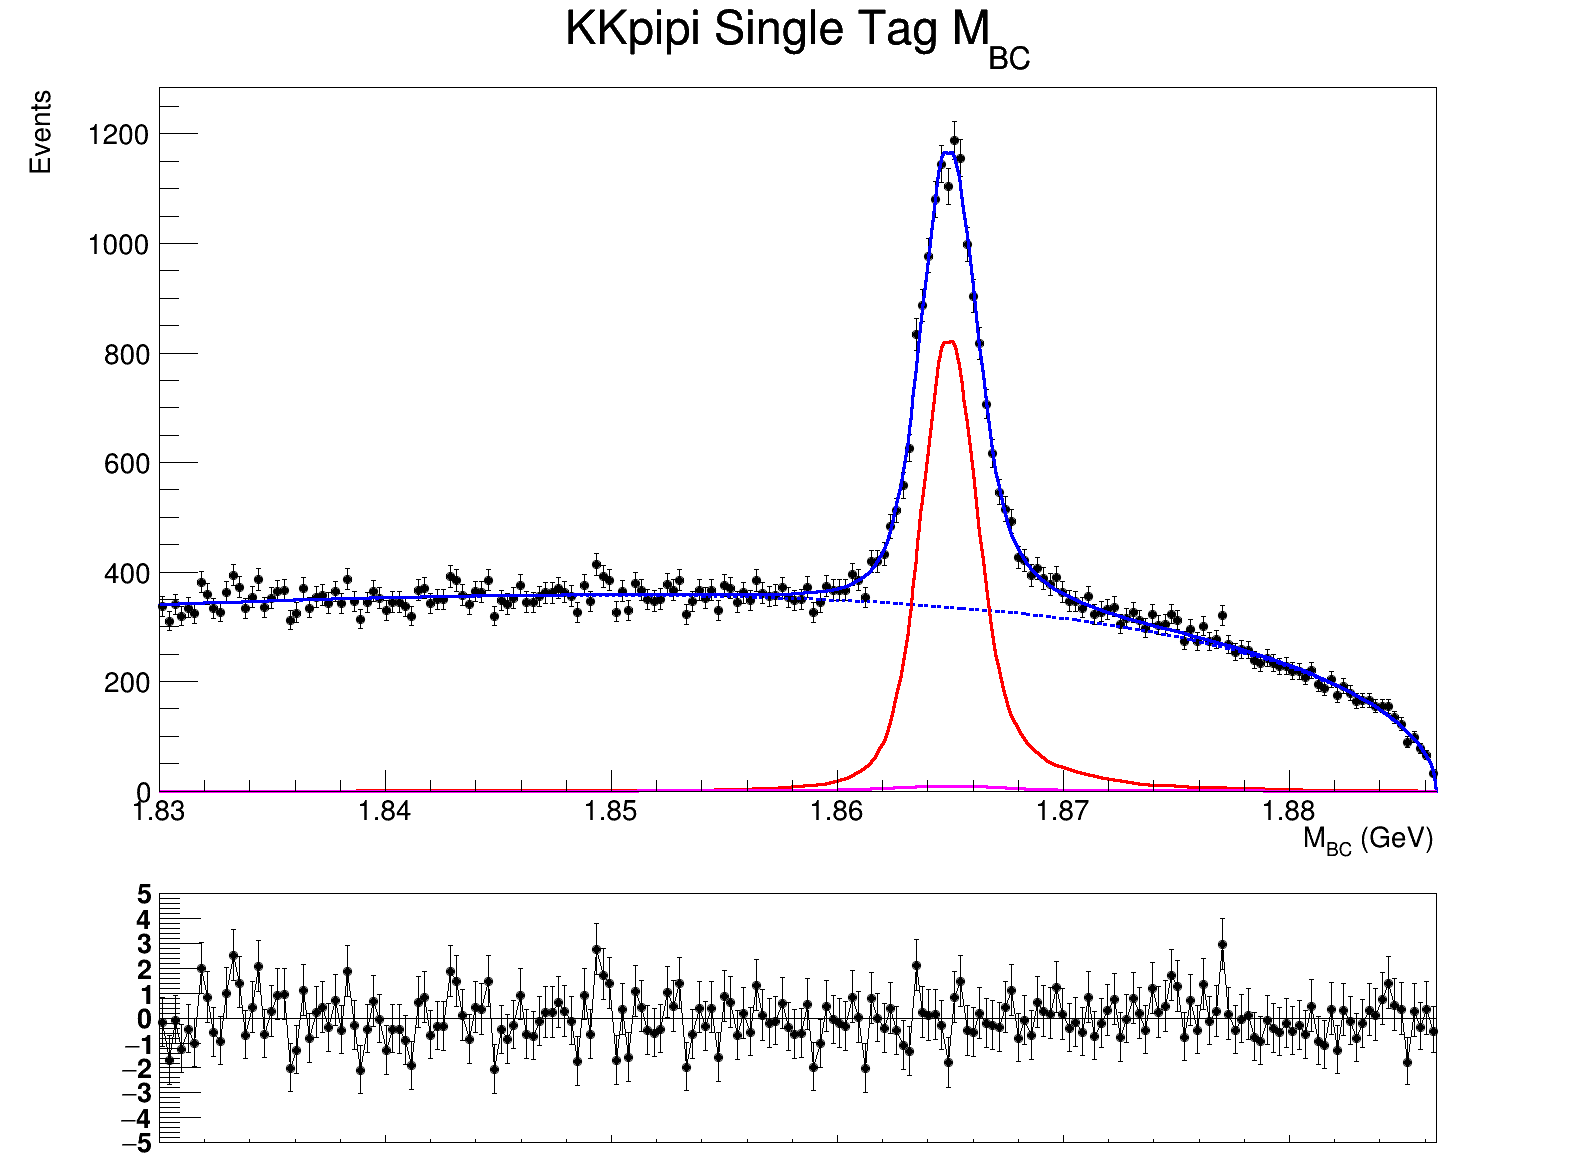
\includegraphics[width=0.65\textwidth]{Plots/KKpipi_SingleTag_MBC_Plot.png}
    \caption{$KK\pi\pi$ single tag fit}
  \end{figure}
\end{frame}

\begin{frame}{Peaking backgrounds}
  \begin{itemize}
    \item{Strategy for fixing peaking backgrounds:}
    \begin{enumerate}
      \item{Generate dedicated MC sample}
      \item{Obtain retention rate of peaking background}
      \item{Fit background with appropriate shape (Gaussian, Crystal Ball, ...)}
      \item{Use BFs from PDG to fix background-to-signal ratio}
    \end{enumerate}
  \end{itemize}
  \begin{figure}
    \centering
    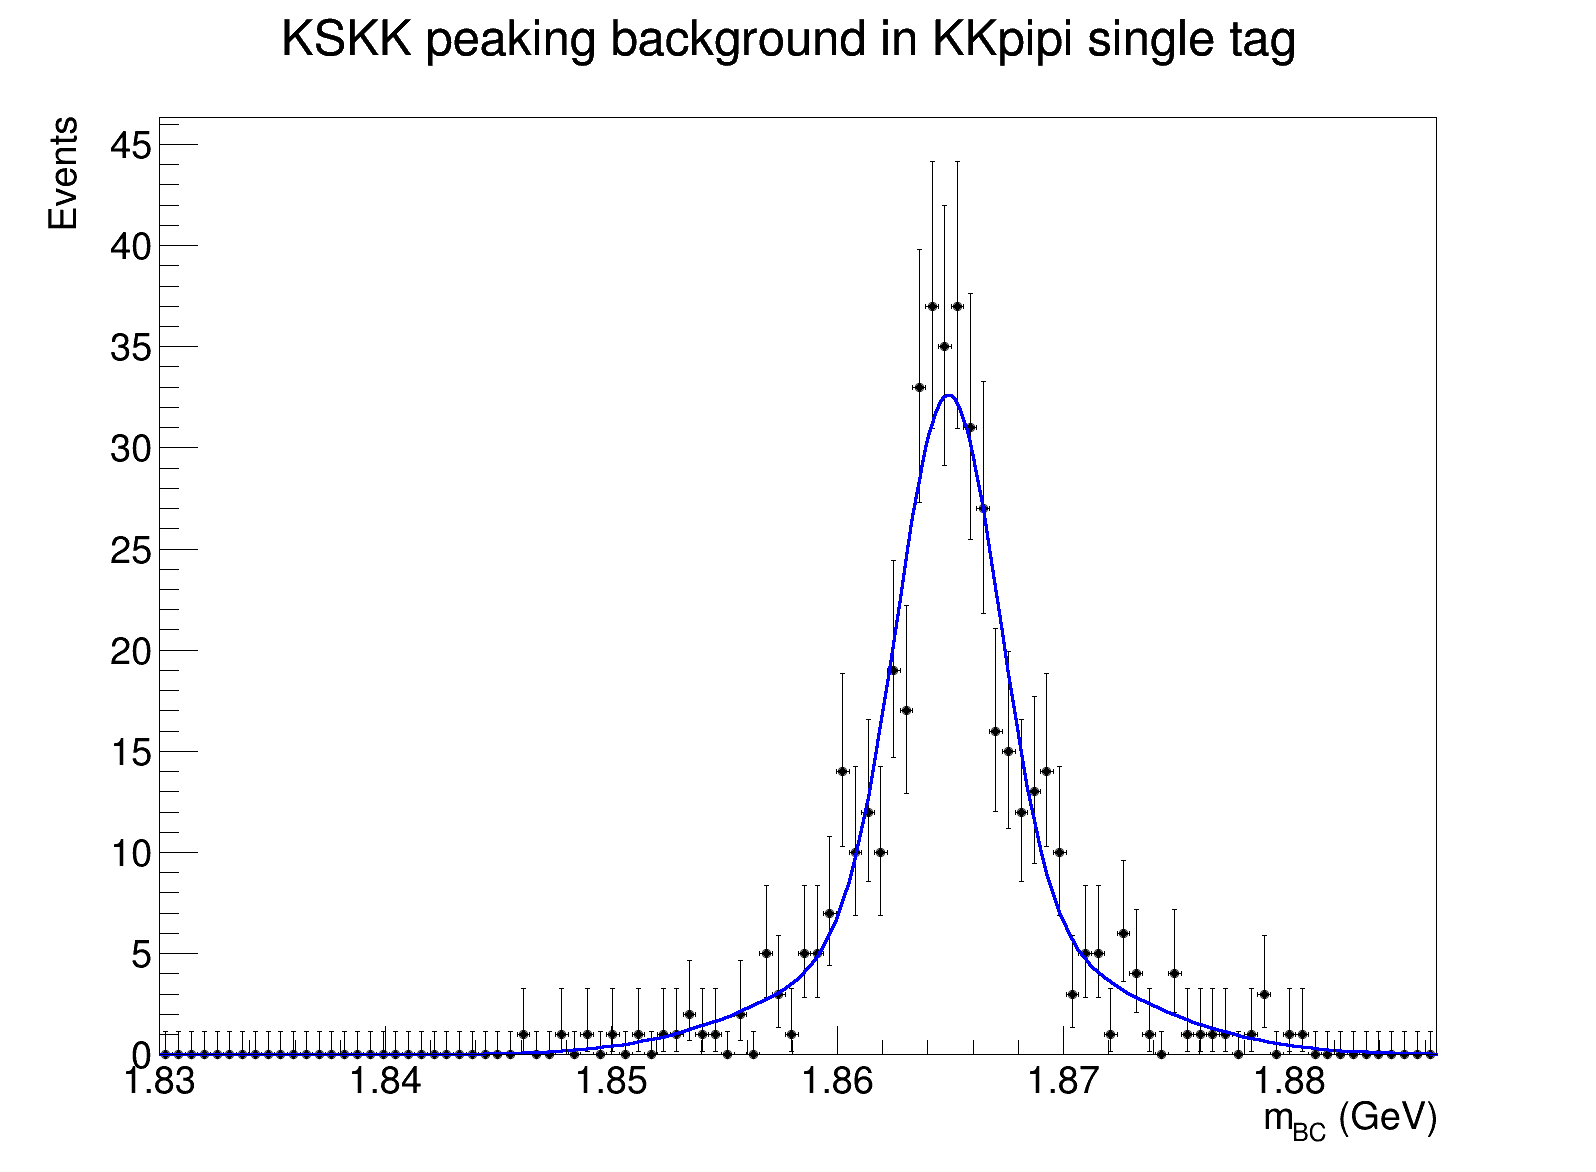
\includegraphics[width=0.50\textwidth]{Plots/KSKKtoKKpipi_Fit.png}
    \caption{$K_SKK$ background in $KK\pi\pi$ single tag fit, fitted with Double Gaussian}
  \end{figure}
\end{frame}

\begin{frame}{Quantum correlation in peaking backgrounds}
  \begin{itemize}
    \item{Strategy for peaking backgrounds with different CP:}
    \begin{itemize}
      \item{Correct using $F_+^{KK\pi\pi}$ from LHCb model}
    \end{itemize}
    \item{Strategy for $K_SKK$ background in $KK\pi\pi$}
    \begin{itemize}
      \item{$F_+^{K_SKK} = \SI{0.524(18)}{}$ from \href{https://arxiv.org/abs/2007.07959}{Phys. Rev. D \textbf{102}, 052008}}
      \item{Use dedicated MC to find retention in each $K_SKK$ bin}
      \item{$K_S$ veto removes more $K_S\phi$ than $K_Sa(980)^0$ $\implies$ Calculate effective $F_+$ for $K_SKK$ to $KK\pi\pi$ background}
    \end{itemize}
  \end{itemize}
  \begin{figure}
    \centering
    \begin{subfigure}{0.5\textwidth}
      \centering
      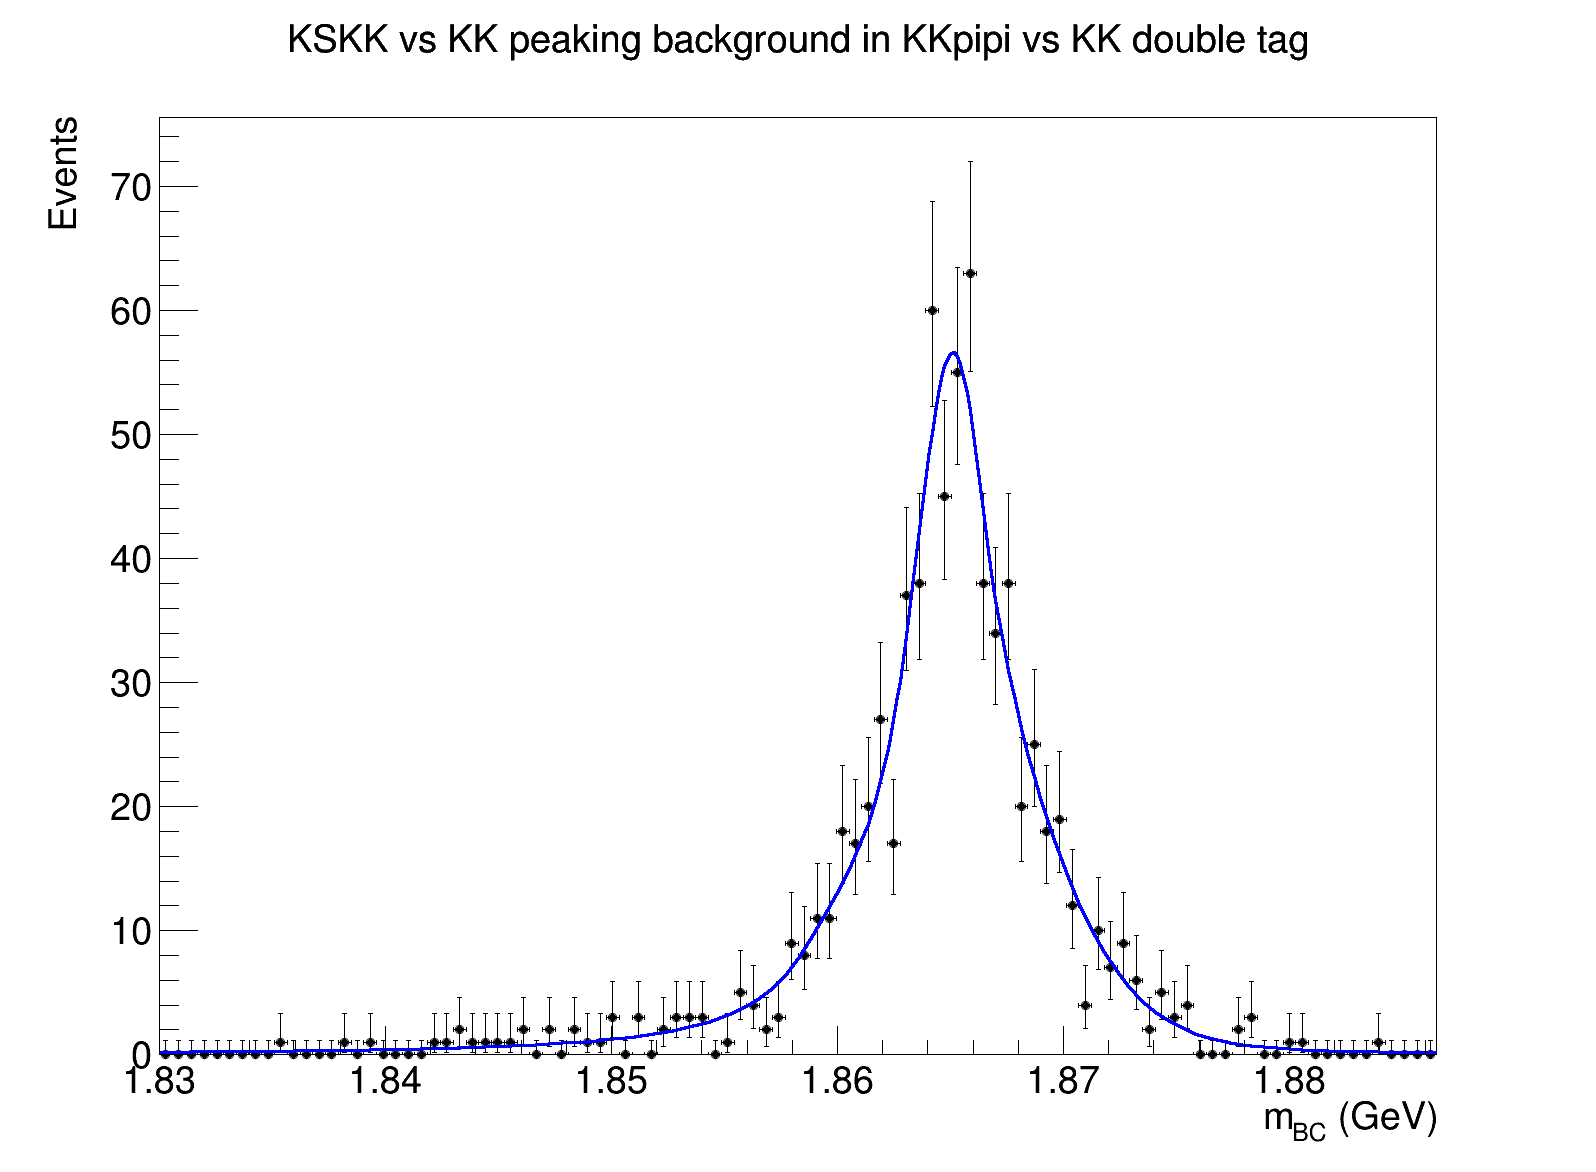
\includegraphics[width=0.95\textwidth]{Plots/KSKK_to_KKpipi_vs_KK_DoubleTag_FitPlot.png}
      \caption{$F_+^{K_SKK} = \SI{0.726(30)}{}$}
    \end{subfigure}%
    \begin{subfigure}{0.5\textwidth}
      \centering
      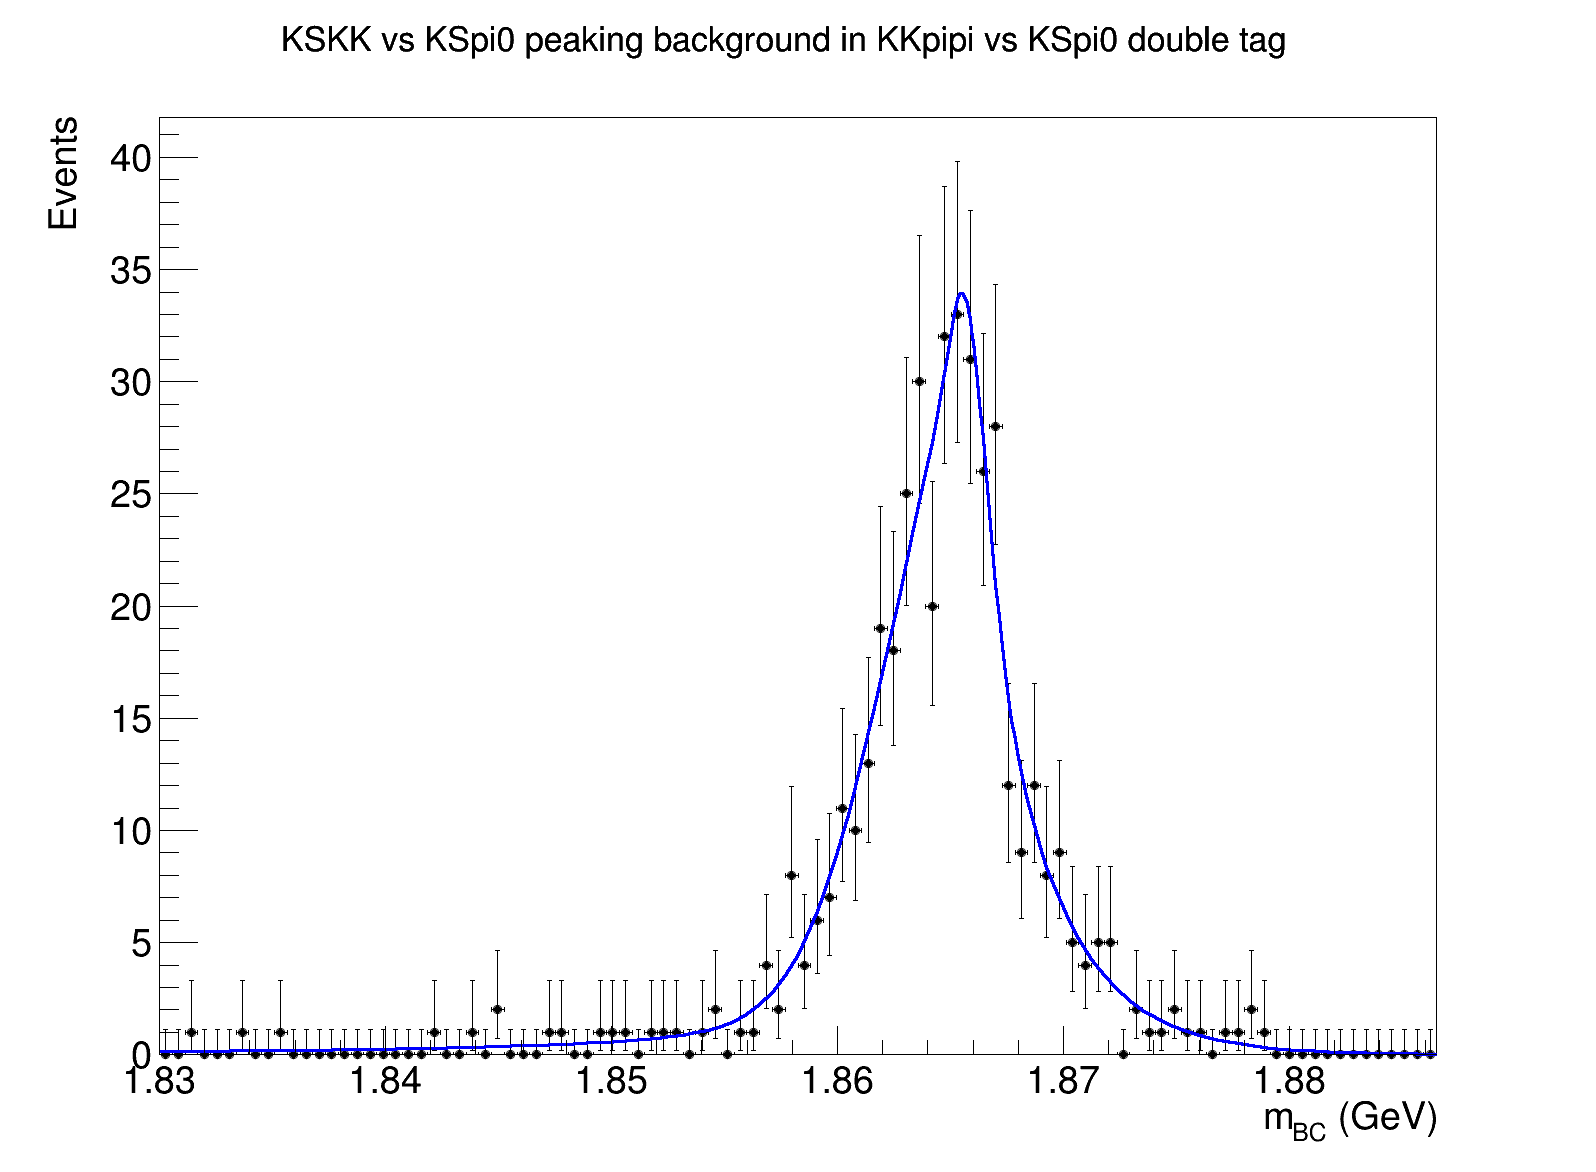
\includegraphics[width=0.95\textwidth]{Plots/KSKK_to_KKpipi_vs_KSpi0_DoubleTag_FitPlot.png}
      \caption{$F_+^{K_SKK} = \SI{0.840(34)}{}$}
    \end{subfigure}
  \end{figure}
\end{frame}

\begin{frame}{Double tag fits}
  \begin{itemize}
    \item{Fit strategy: Only fit signal side $m_{\rm BC}$ because of low statistics}
    \item{Fit model:}
    \begin{itemize}
      \item{Signal: PDF from signal MC, convoluted with single Gaussian}
      \item{Background: Argus PDF}
      \item{Simple sideband subtraction for correct signal but wrong tag event}
    \end{itemize}
    \item{For tags with multiple bins, perform a simultaneous fit of all bins}
    \begin{itemize}
      \item{Shape is floated and shared across all bins}
      \item{Yield of signal and combinatorial background is floated in each bin}
    \end{itemize}
  \end{itemize}
  \begin{figure}
    \centering
    \begin{subfigure}{0.5\textwidth}
      \centering
      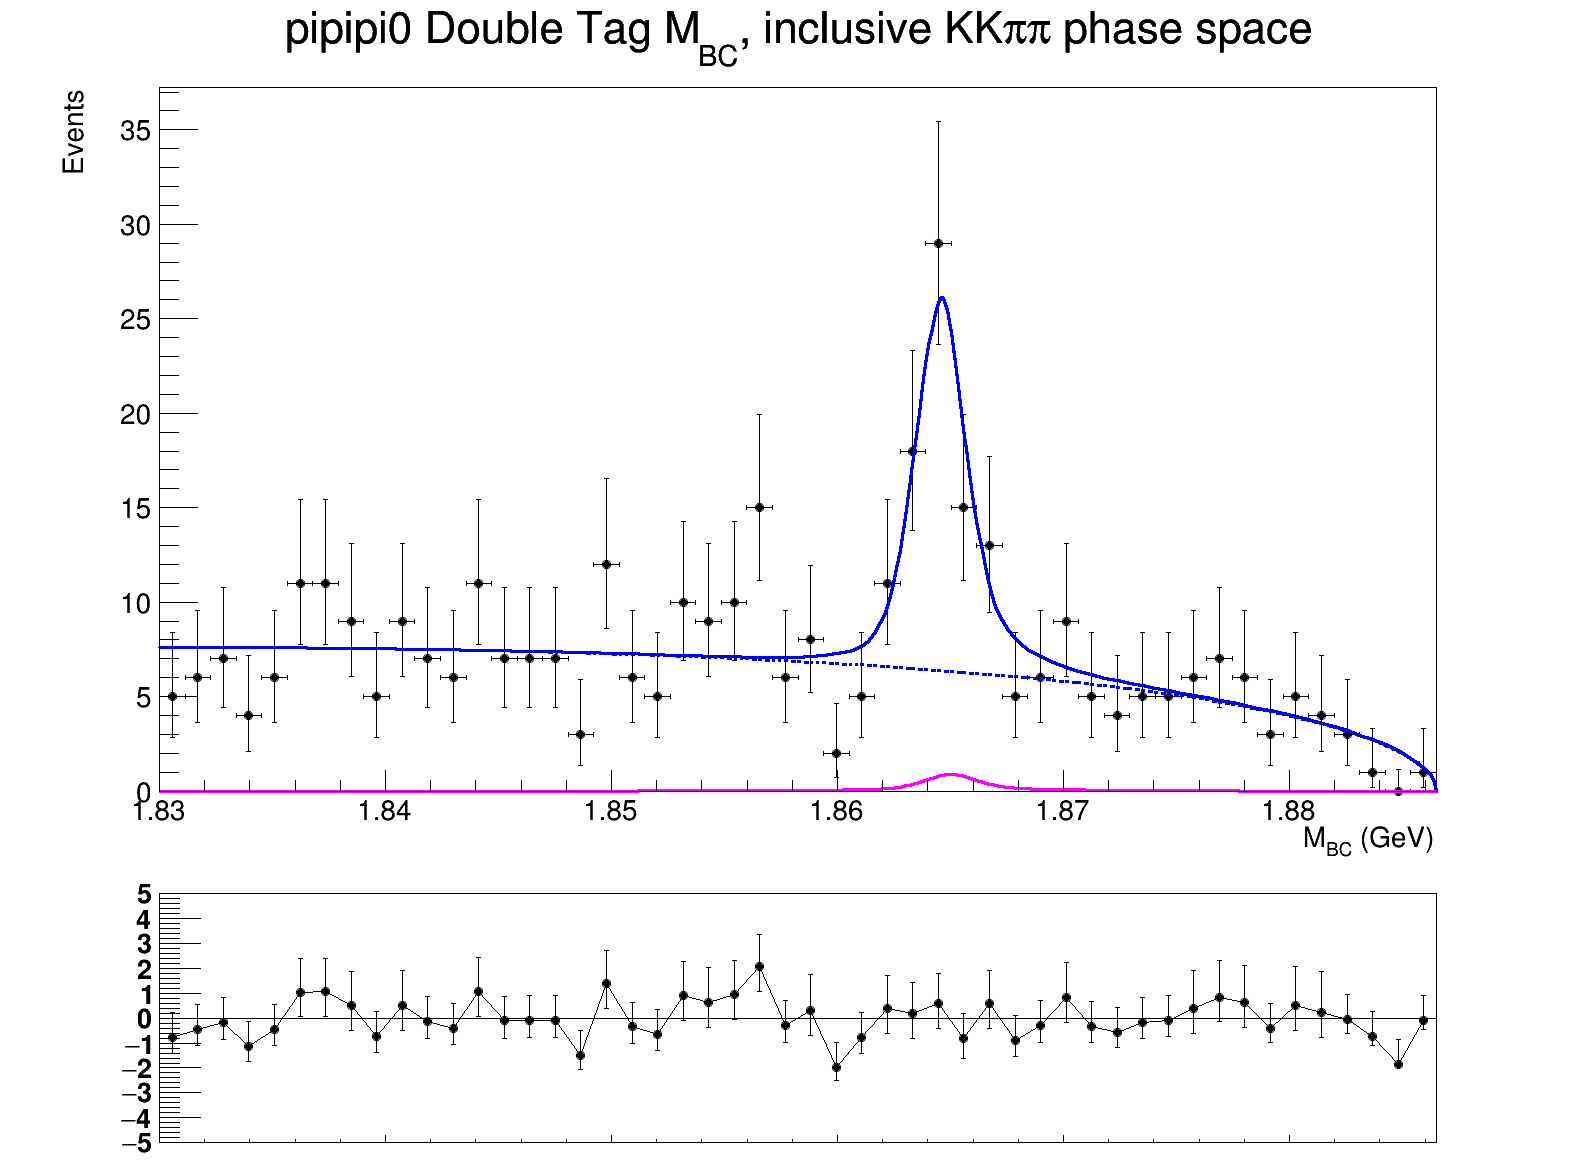
\includegraphics[width=0.85\textwidth]{Plots/DoubleTagYield_DoubleTag_CP_KKpipi_vs_pipipi0_SignalBin0.png}
      \caption{$KK\pi\pi$ vs $\pi\pi\pi^0$}
    \end{subfigure}%
    \begin{subfigure}{0.5\textwidth}
      \centering
      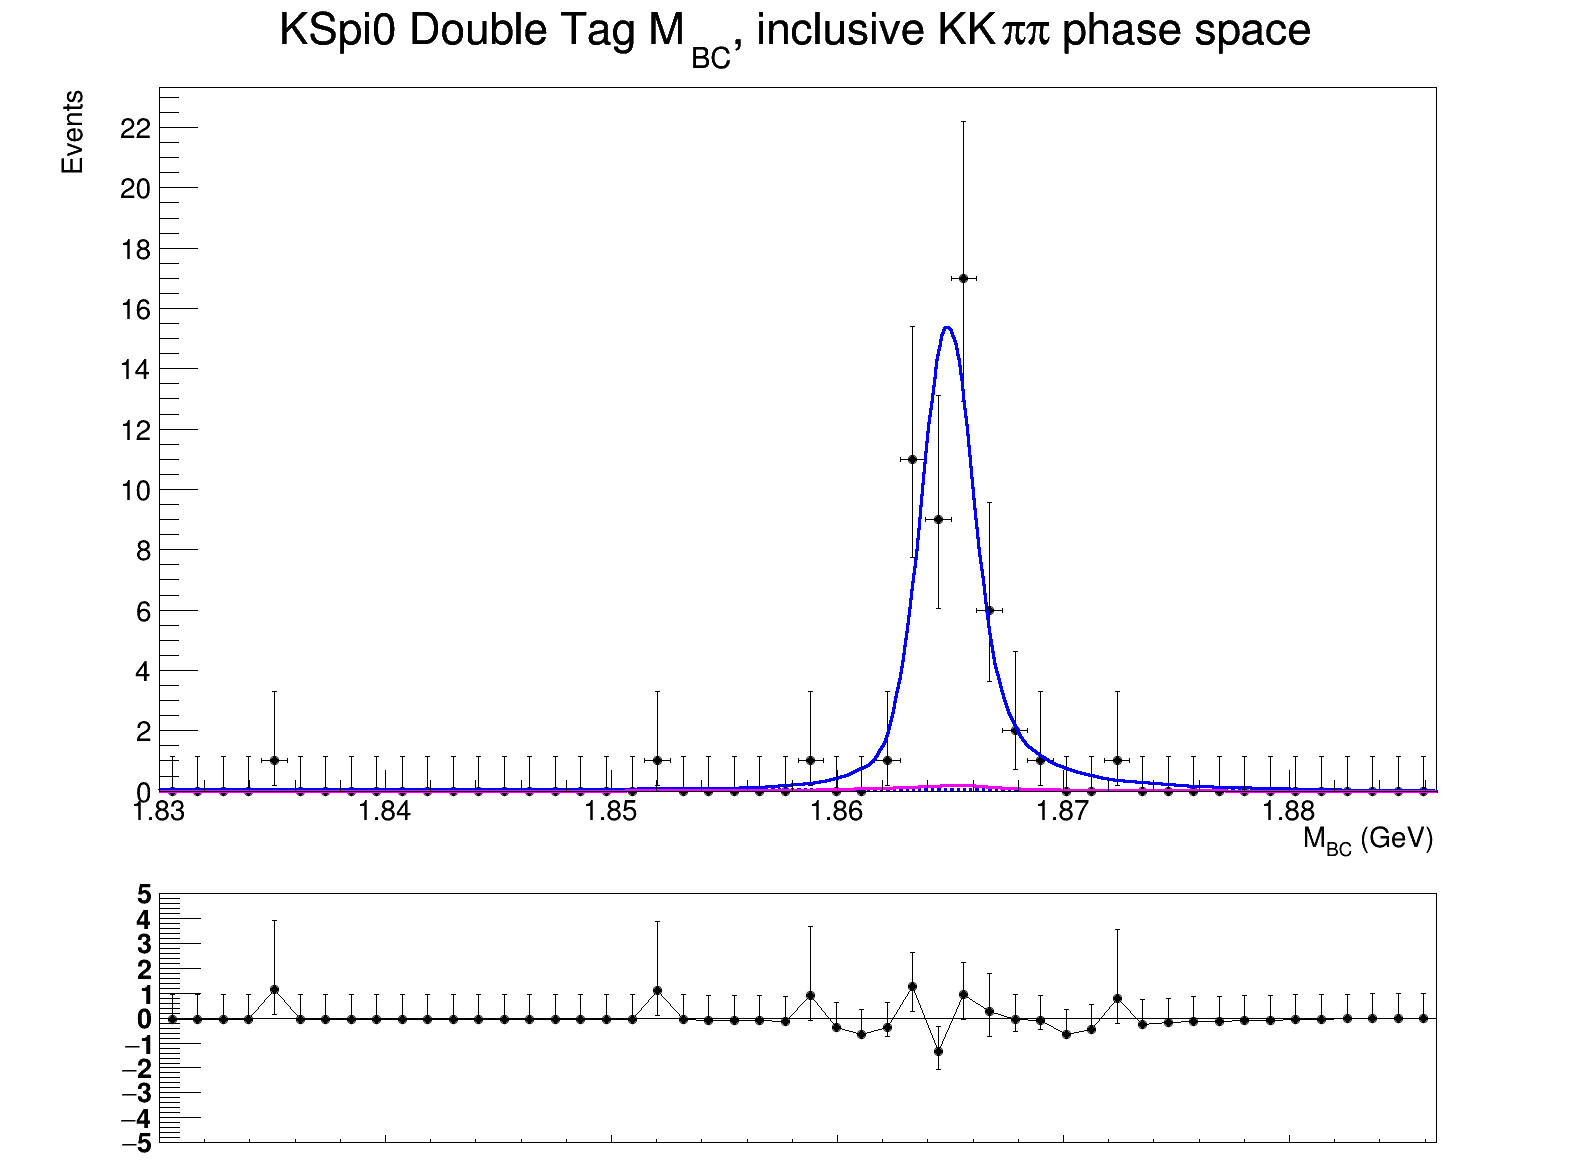
\includegraphics[width=0.85\textwidth]{Plots/DoubleTagYield_DoubleTag_CP_KKpipi_vs_KSpi0_SignalBin0.png}
      \caption{$KK\pi\pi$ vs $K_S\pi^0$}
    \end{subfigure}
  \end{figure}
\end{frame}

\begin{frame}{Double tag fits}
  \begin{figure}
    \centering
    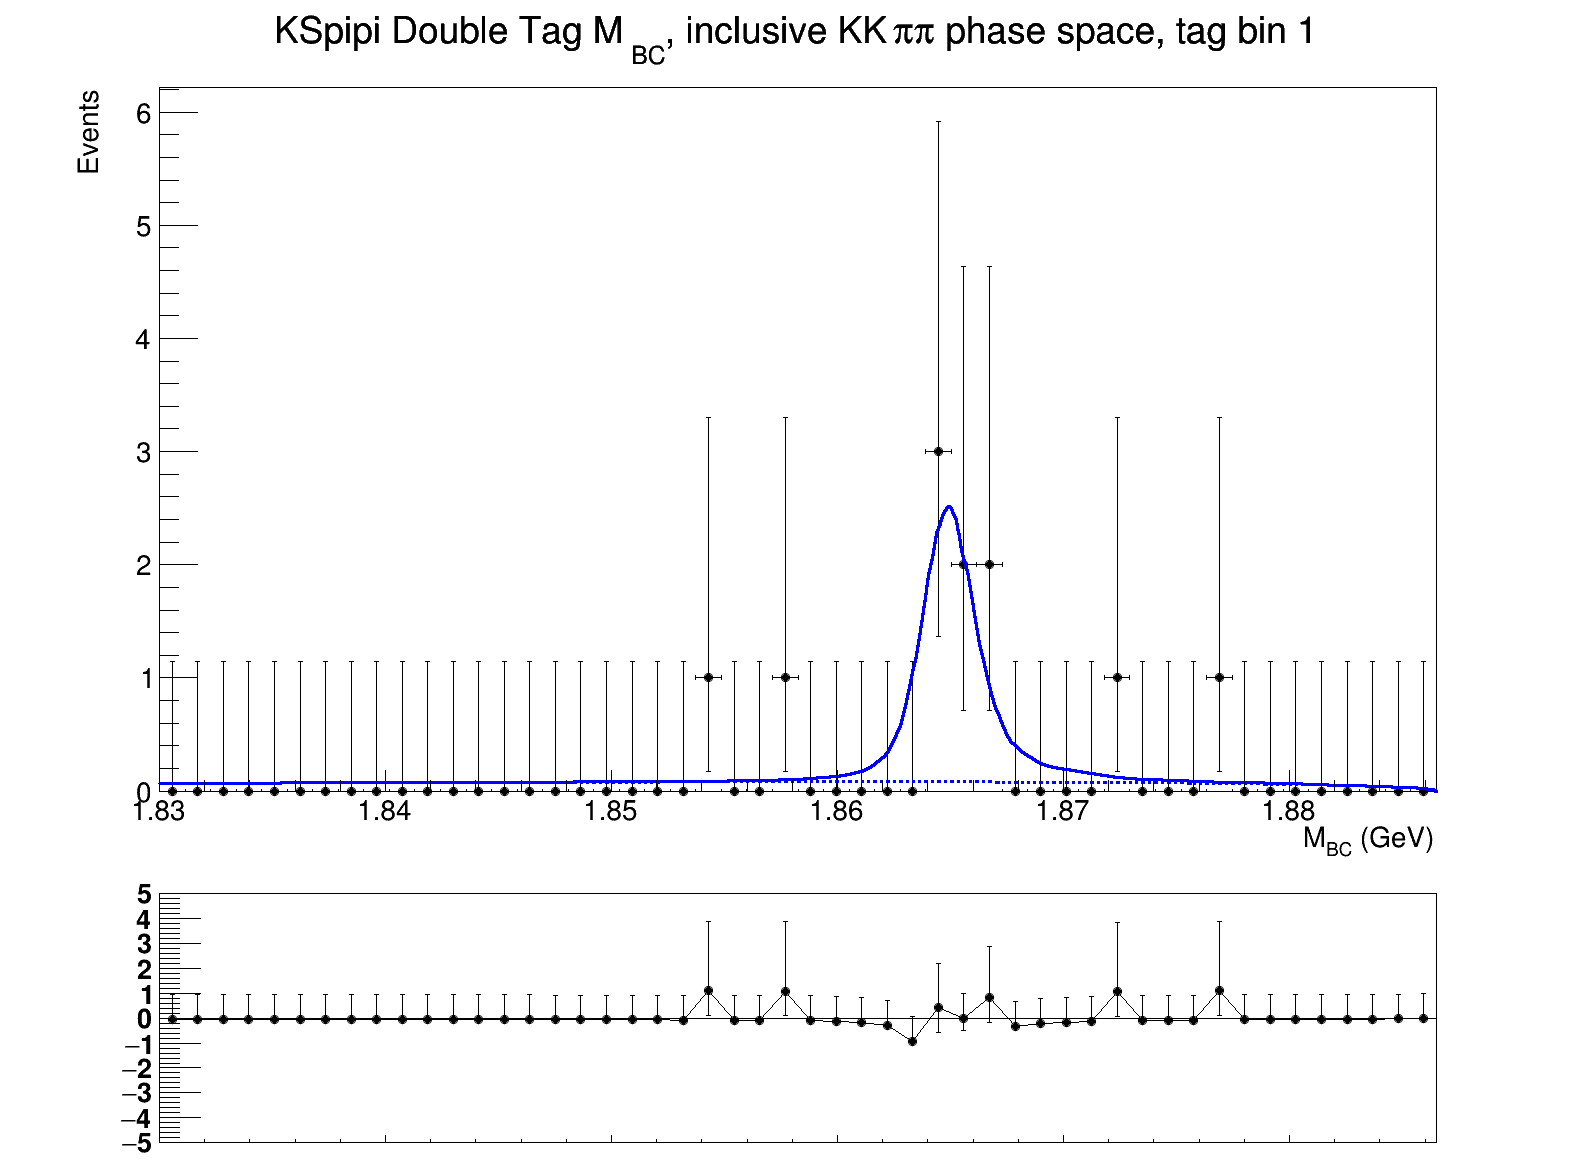
\includegraphics[width=0.32\textwidth, clip = true, trim = {0 11cm 0 0}]{Plots/DoubleTagYield_DoubleTag_SCMB_KKpipi_vs_KSpipi_SignalBin0_TagBin1.png}
    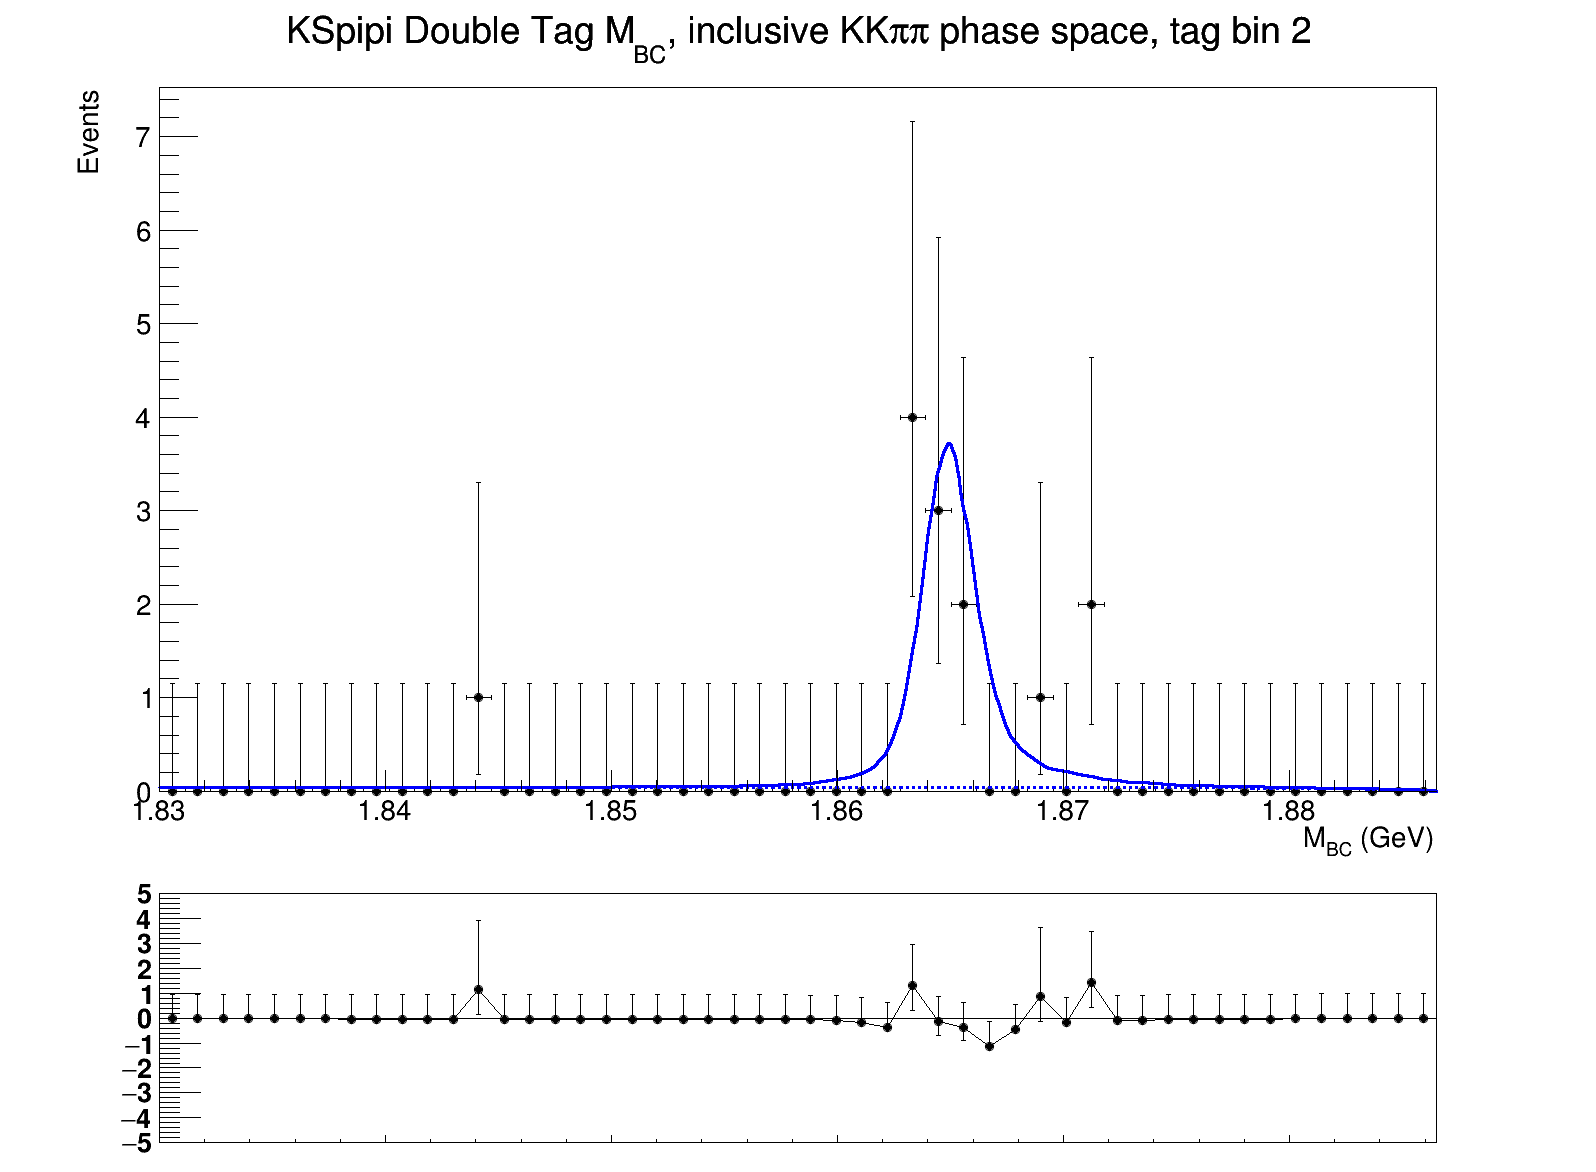
\includegraphics[width=0.32\textwidth, clip = true, trim = {0 11cm 0 0}]{Plots/DoubleTagYield_DoubleTag_SCMB_KKpipi_vs_KSpipi_SignalBin0_TagBin2.png}
    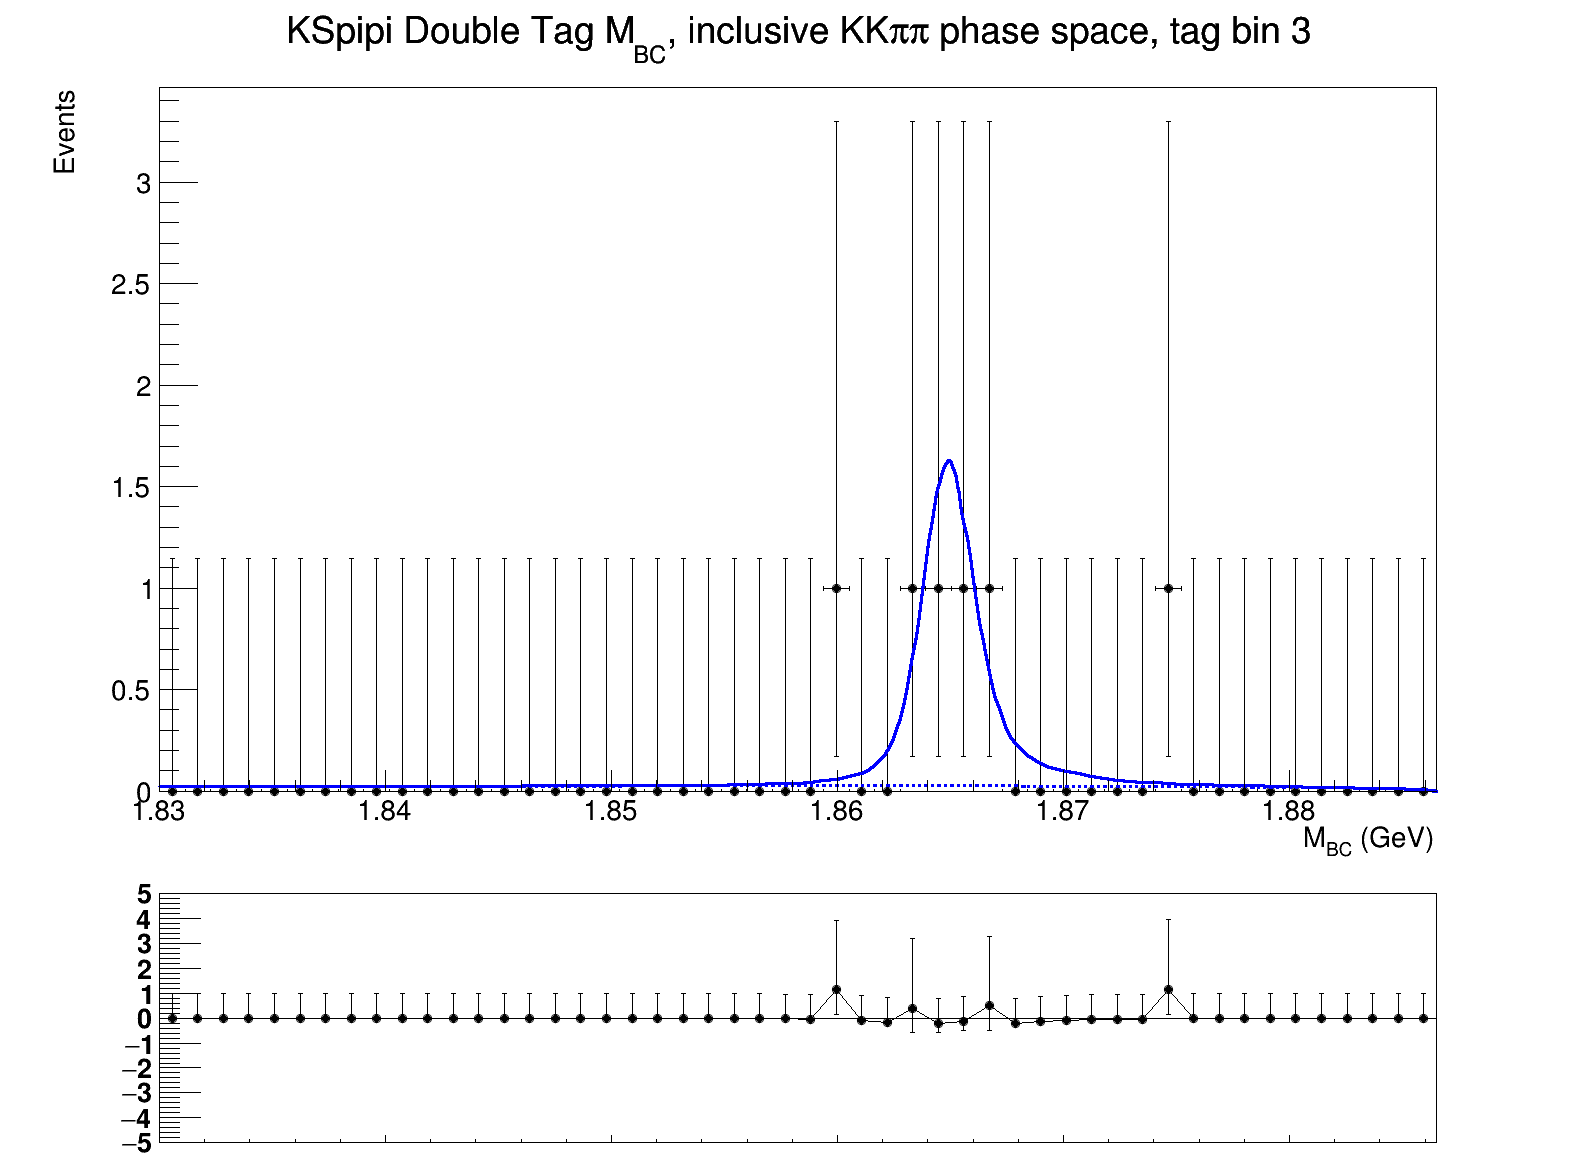
\includegraphics[width=0.32\textwidth, clip = true, trim = {0 11cm 0 0}]{Plots/DoubleTagYield_DoubleTag_SCMB_KKpipi_vs_KSpipi_SignalBin0_TagBin3.png}
    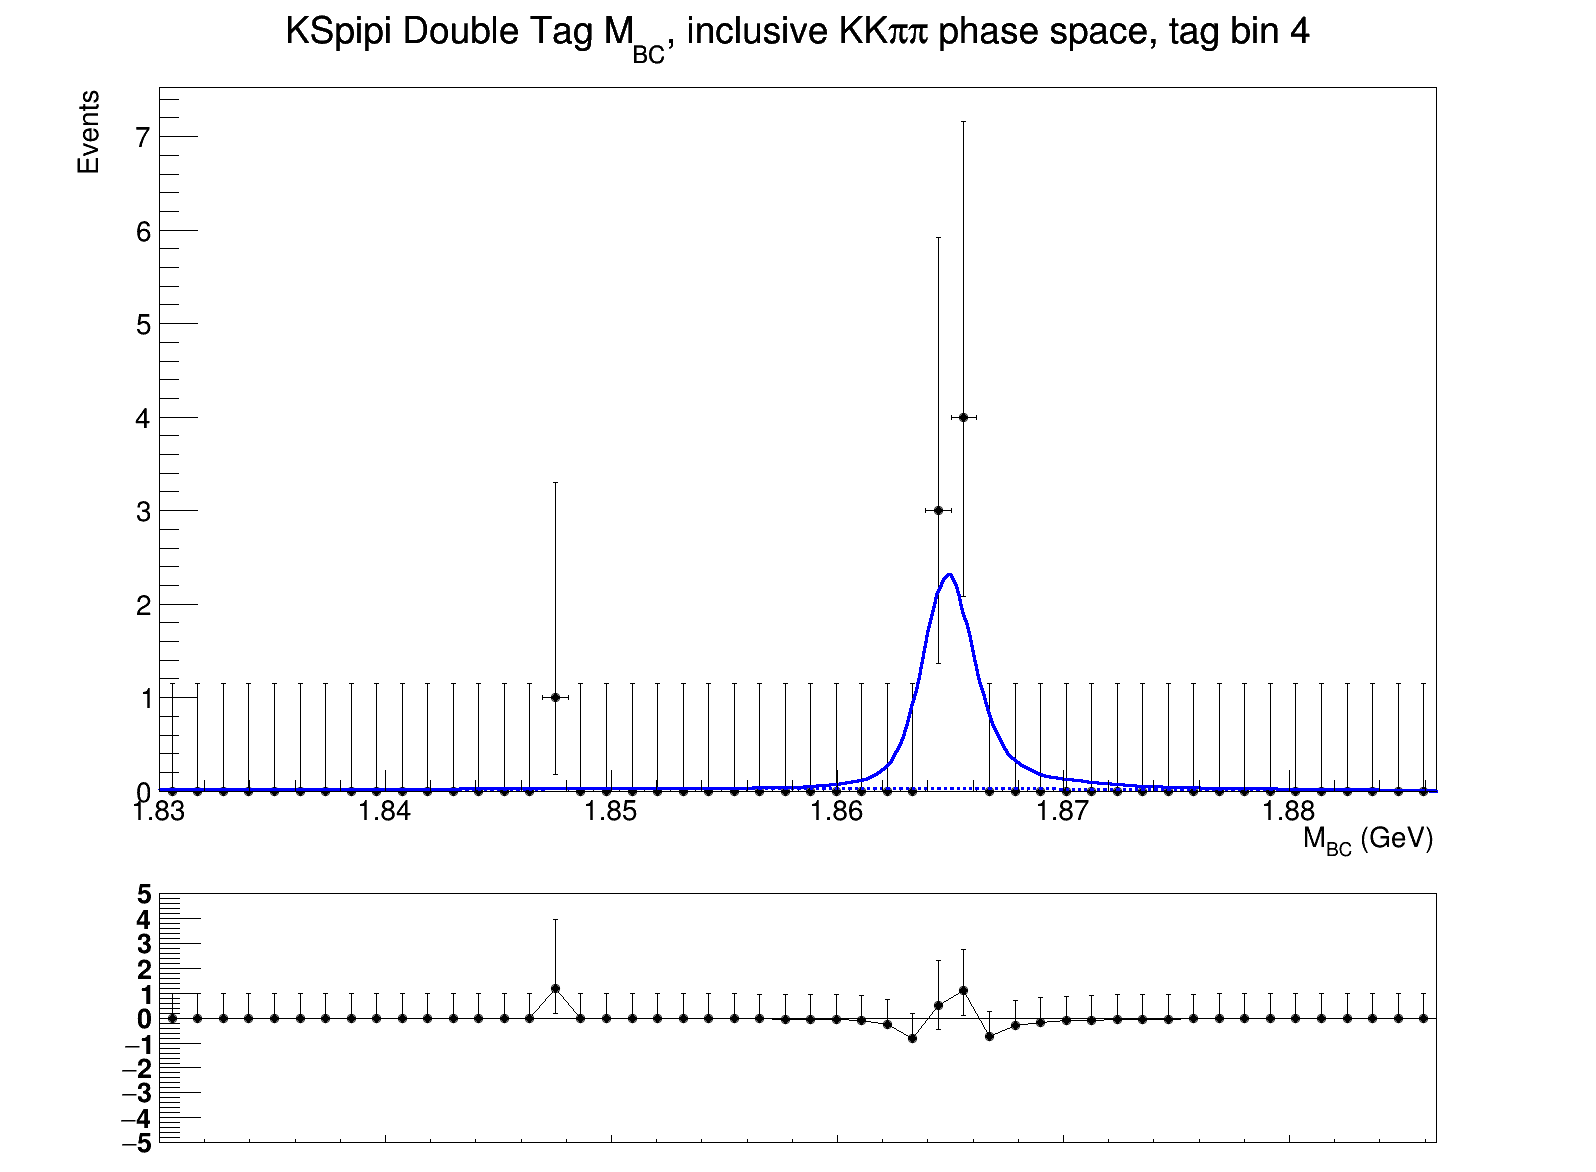
\includegraphics[width=0.32\textwidth, clip = true, trim = {0 11cm 0 0}]{Plots/DoubleTagYield_DoubleTag_SCMB_KKpipi_vs_KSpipi_SignalBin0_TagBin4.png}
    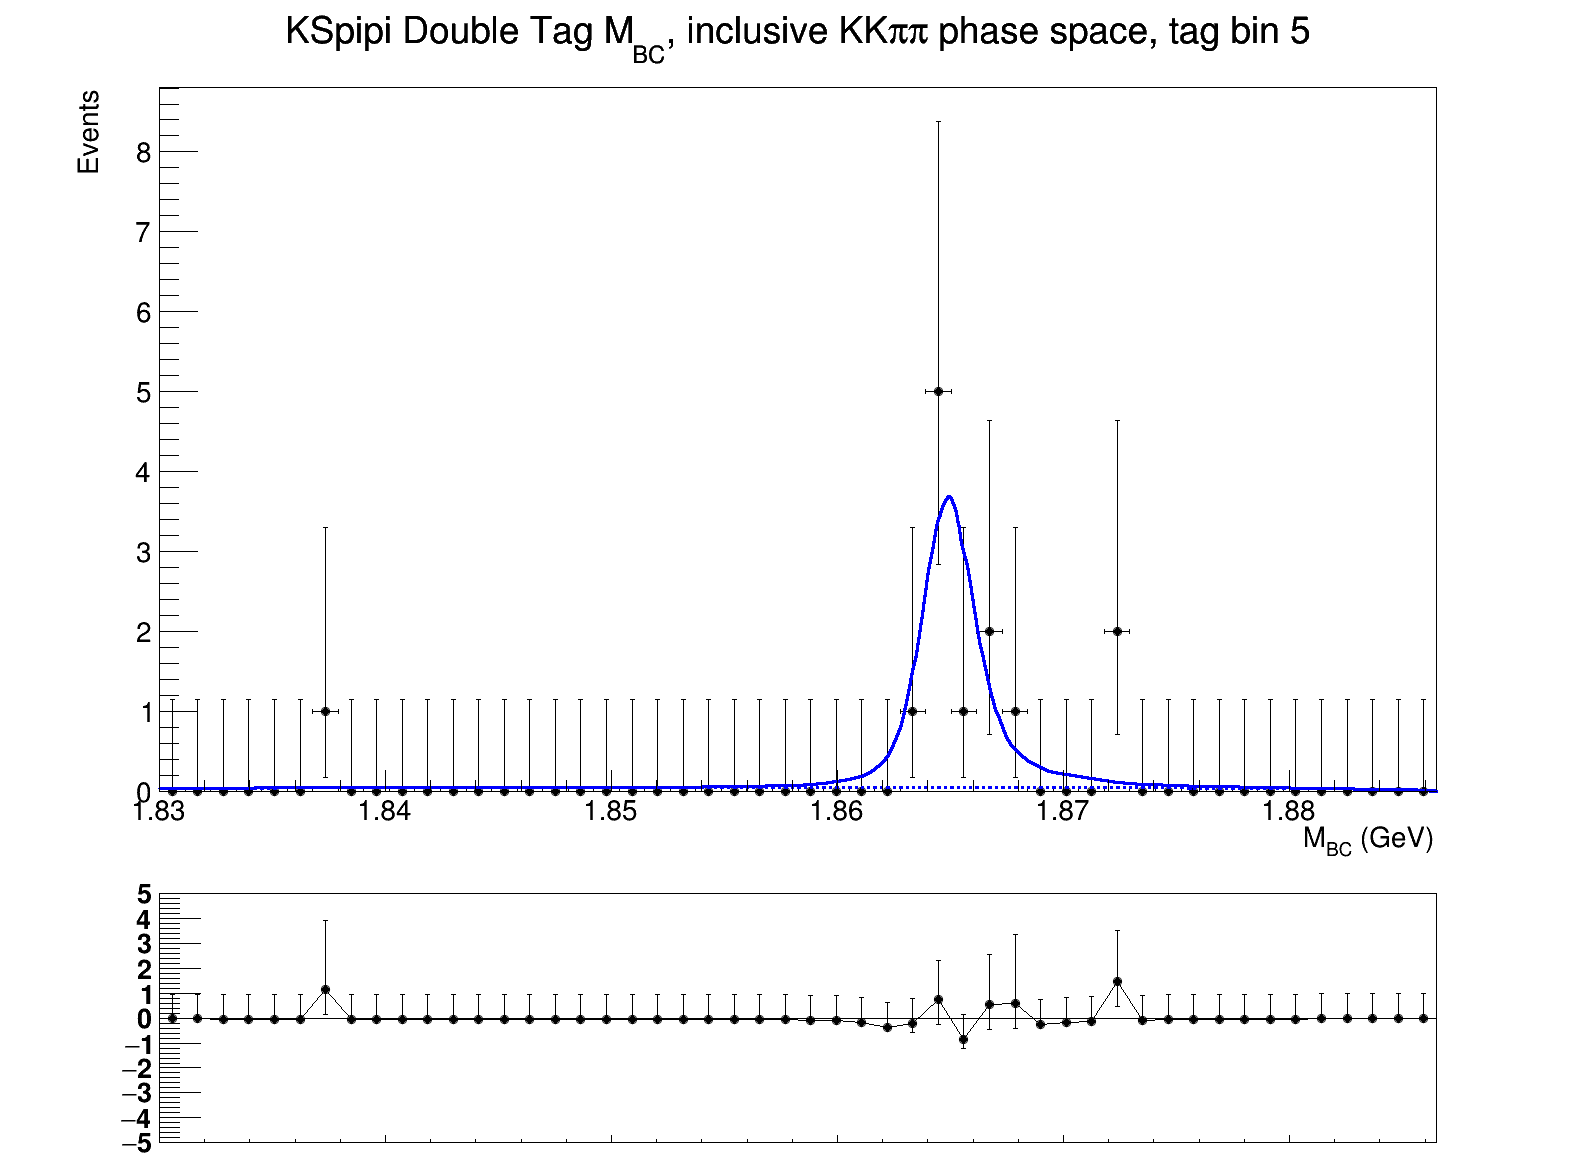
\includegraphics[width=0.32\textwidth, clip = true, trim = {0 11cm 0 0}]{Plots/DoubleTagYield_DoubleTag_SCMB_KKpipi_vs_KSpipi_SignalBin0_TagBin5.png}
    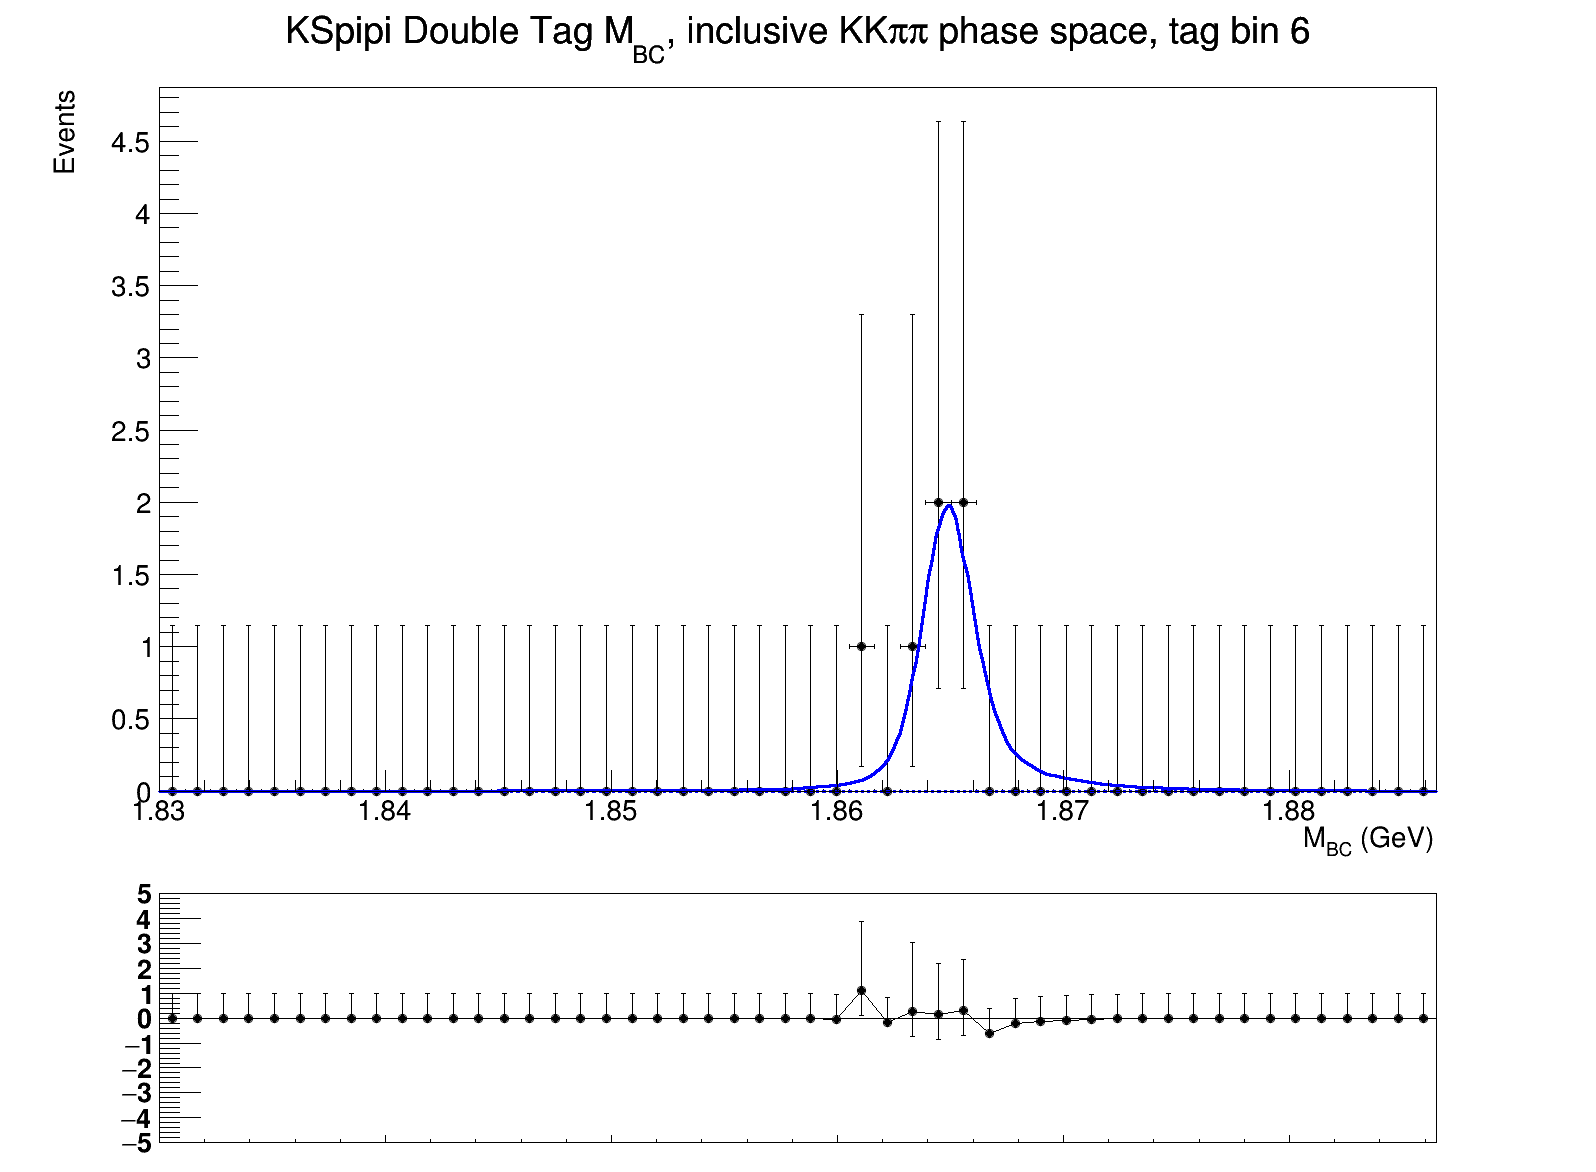
\includegraphics[width=0.32\textwidth, clip = true, trim = {0 11cm 0 0}]{Plots/DoubleTagYield_DoubleTag_SCMB_KKpipi_vs_KSpipi_SignalBin0_TagBin6.png}
    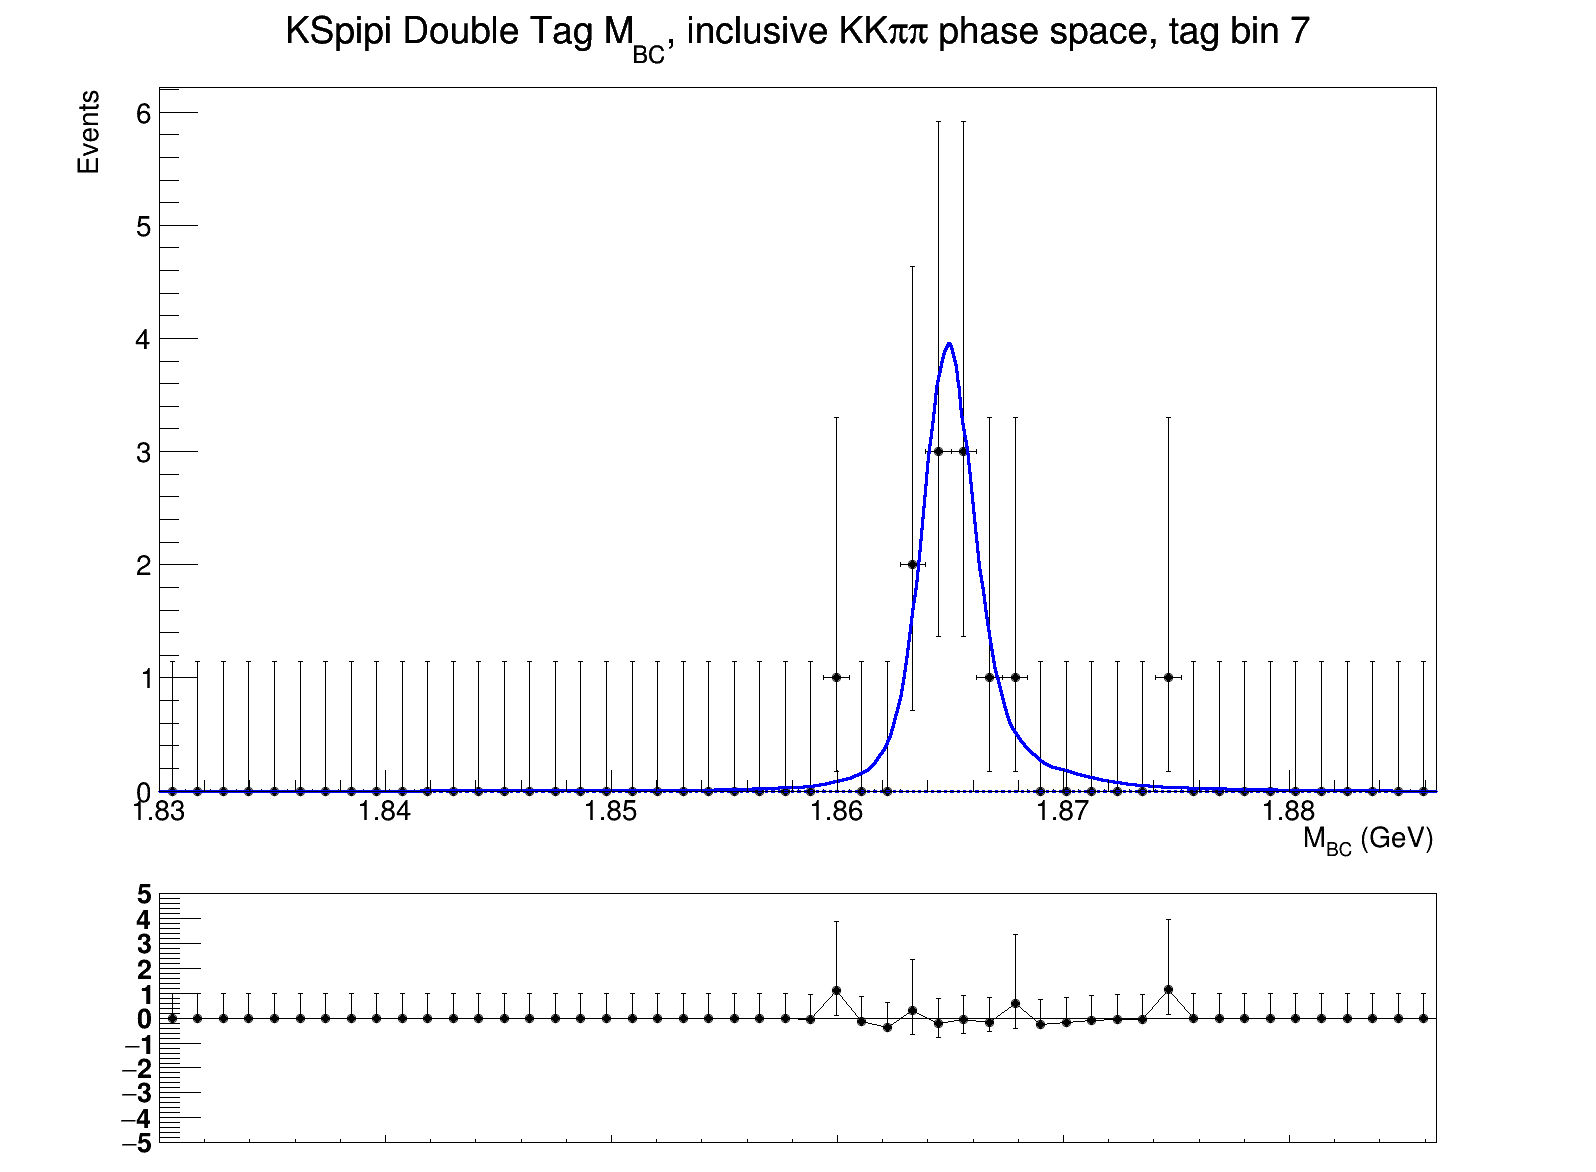
\includegraphics[width=0.32\textwidth, clip = true, trim = {0 11cm 0 0}]{Plots/DoubleTagYield_DoubleTag_SCMB_KKpipi_vs_KSpipi_SignalBin0_TagBin7.png}
    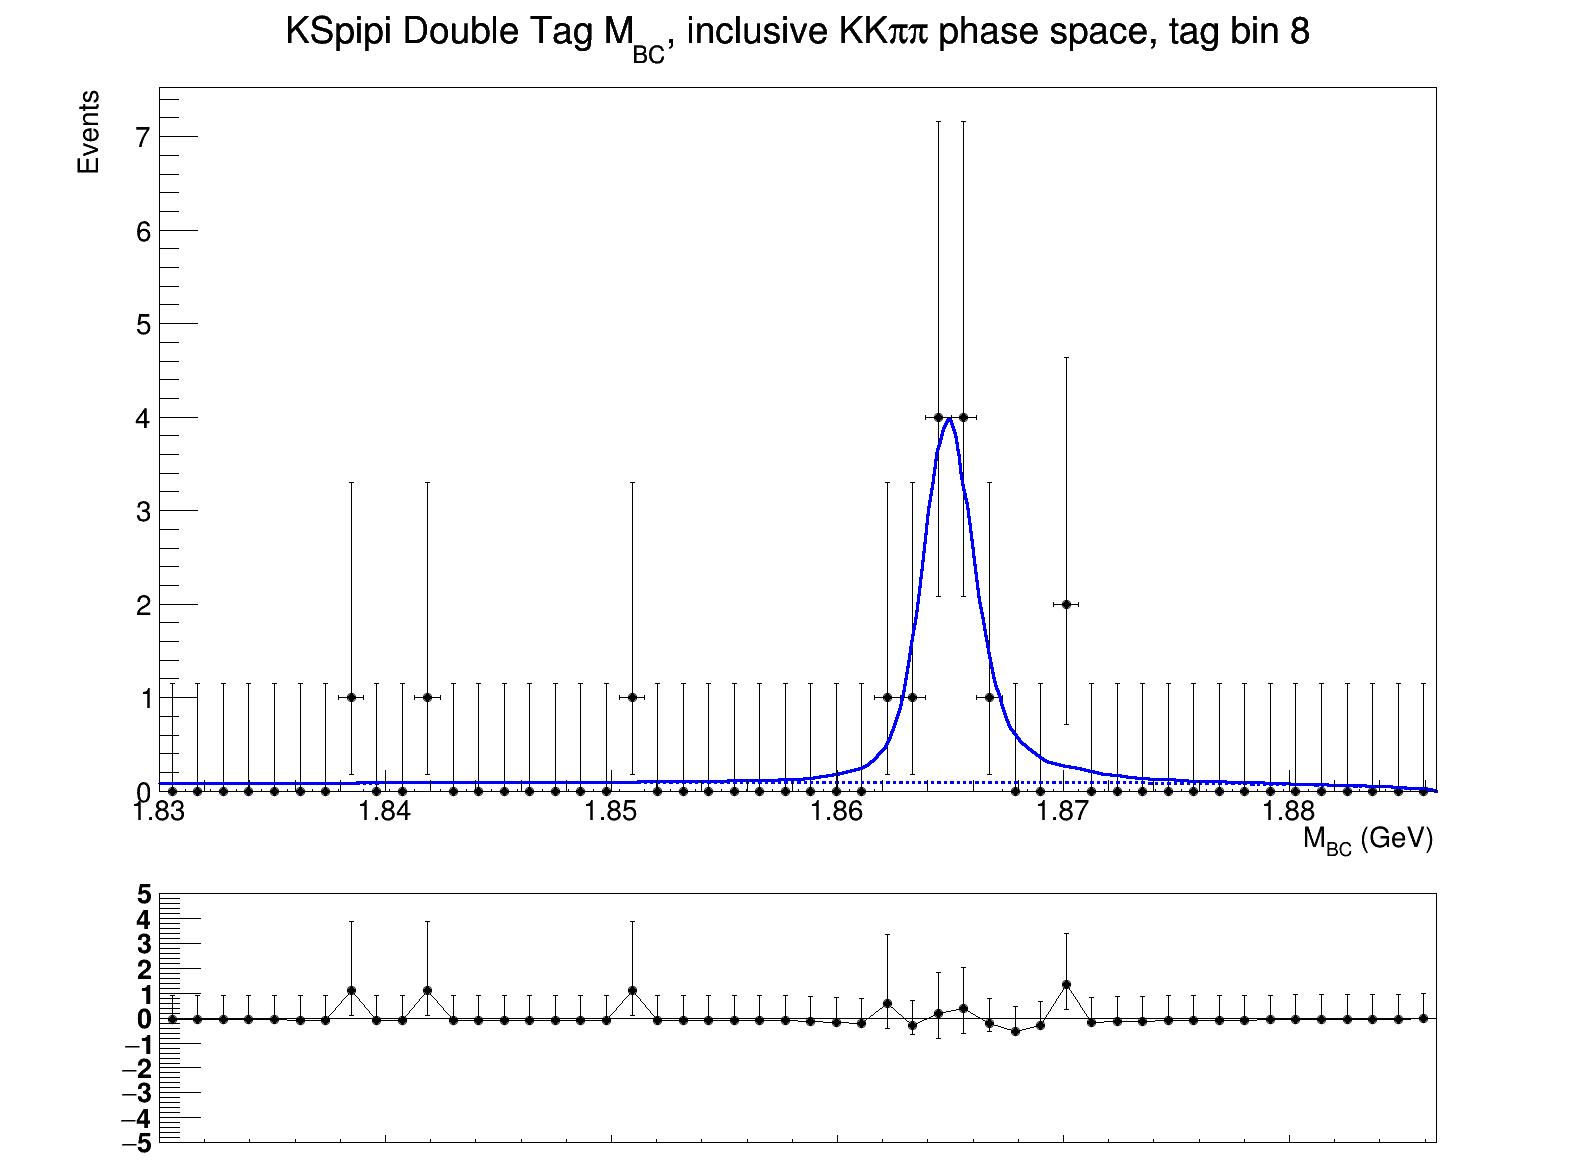
\includegraphics[width=0.32\textwidth, clip = true, trim = {0 11cm 0 0}]{Plots/DoubleTagYield_DoubleTag_SCMB_KKpipi_vs_KSpipi_SignalBin0_TagBin8.png}
    \caption{$KK\pi\pi$ vs $K_S\pi\pi$ simultaneous fit}
  \end{figure}
\end{frame}

\begin{frame}{Initial look at $K_i$ for $D^0\to KK\pi\pi$}
  \begin{itemize}
    \item{Expect fractional bin yields $K_i$ to be well described by LHCb model}
    \item{$K_i$ are accessible at LHCb in $B\to D\mu X$ processes with large statistics}
    \item{Excellent agreement between model and data!}
  \end{itemize}
  \begin{figure}
    \centering
    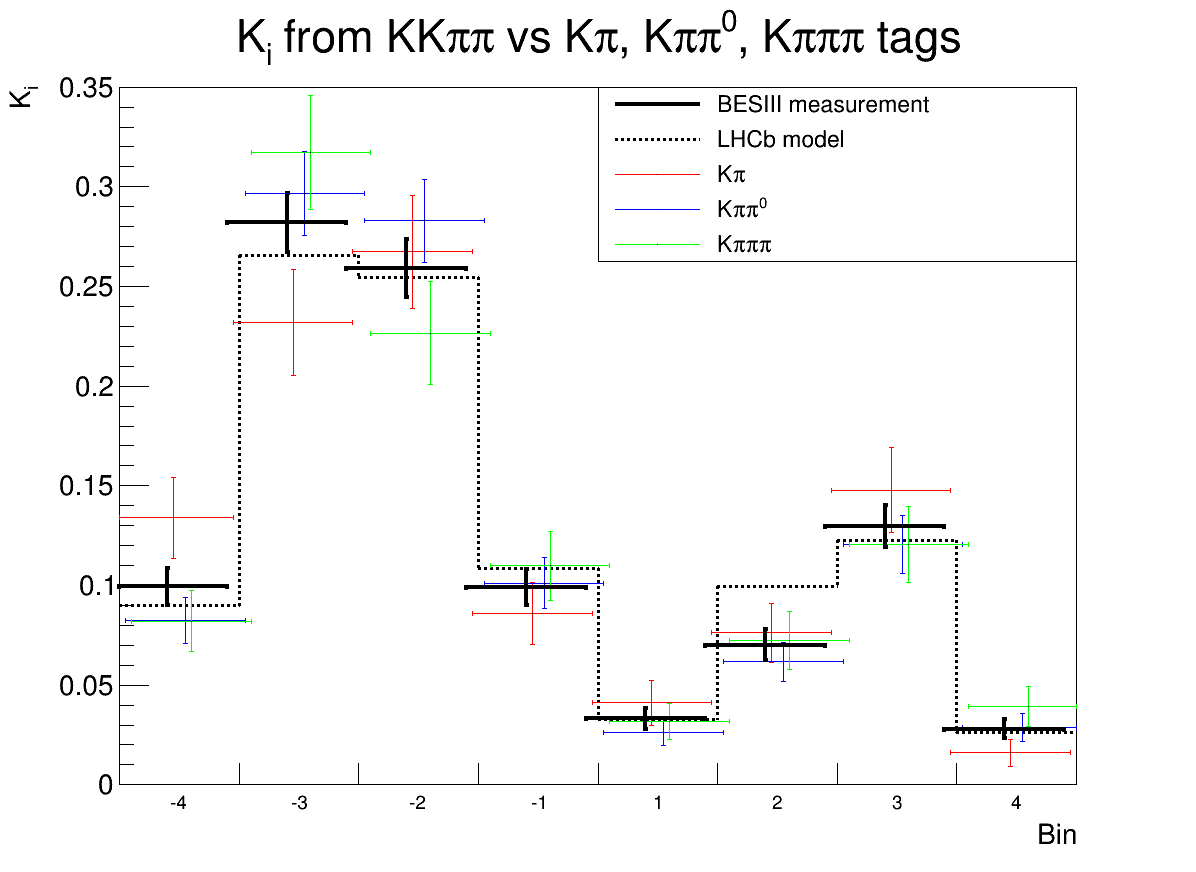
\includegraphics[width=0.65\textwidth]{Plots/Ki_Measured_vs_Model.png}
    \caption{$K_i$ measurement for $KK\pi\pi$ using $2\times 4$ bins}
  \end{figure}
\end{frame}

\section{\texorpdfstring{$F_+$}{F+} measurement}
\subsection{With CP tags}
\begin{frame}{$F_+$ measurement with CP tags}
  \begin{itemize}
    \item{Normalize double tag yields with single tag yields:}
  \end{itemize}
  \begin{equation*}
    \frac{N_{\rm DT}(KK\pi\pi|\text{tag})}{N_{\rm ST}(\text{tag})}\frac{\epsilon(\text{tag})}{\epsilon(KK\pi\pi|\text{tag})} = \text{BF}(KK\pi\pi)\big(1 - 2(2F_+^{KK\pi\pi} - 1)(2F_+^{\rm tag} - 1)\big)
  \end{equation*}
  \begin{itemize}
    \item{Fit all CP tags simultaneously with $\text{BF}(KK\pi\pi)$ and $F_+^{KK\pi\pi}$ floated}
  \end{itemize}
  \centering
  %\def\arraystretch{1.2}%
  \small
  \begin{tabular}{l|c|c}
    Mode                          & Single tag yield & Double tag yield \\
    \hline
    $KK$                          & $\SI{56303(262)}{}$   & $\SI{26(6)}{}$ \\
    $\pi\pi$                      & $\SI{19771(130)}{}$   & $\SI{4(4)}{}$ \\
    $\pi\pi\pi^0$                 & $\SI{113780(644)}{}$  & $\SI{56(10)}{}$ \\
    $K_S\pi^0\pi^0$               & $\SI{25122(331)}{}$   & $\SI{8.5(29)}{}$ \\
    $K_L\pi^0$                    & $\SI{48148(463)}{}$   & $\SI{6(4)}{}$ \\
    \hline
    $K_S\pi^0$                    & $\SI{68230(280)}{}$   & $\SI{48(7)}{}$ \\
    $K_S\eta$                     & $\SI{9296(33)}{}$     & $\SI{8.8(29)}{}$ \\
    $K_S\eta^\prime_{\pi\pi\eta}$ & $\SI{3220(6)}{}$      & $\SI{2.2(16)}{}$ \\
    $K_S\eta^\prime_{\rho\gamma}$ & $\SI{8740(196)}{}$    & $\SI{8.9(30)}{}$ \\
    $K_S\omega$                   & $\SI{21636(170)}{}$   & $\SI{10(4)}{}$ \\
  \end{tabular}
\end{frame}

\begin{frame}{$F_+$ measurement with CP tags}
  \begin{figure}
    \centering
    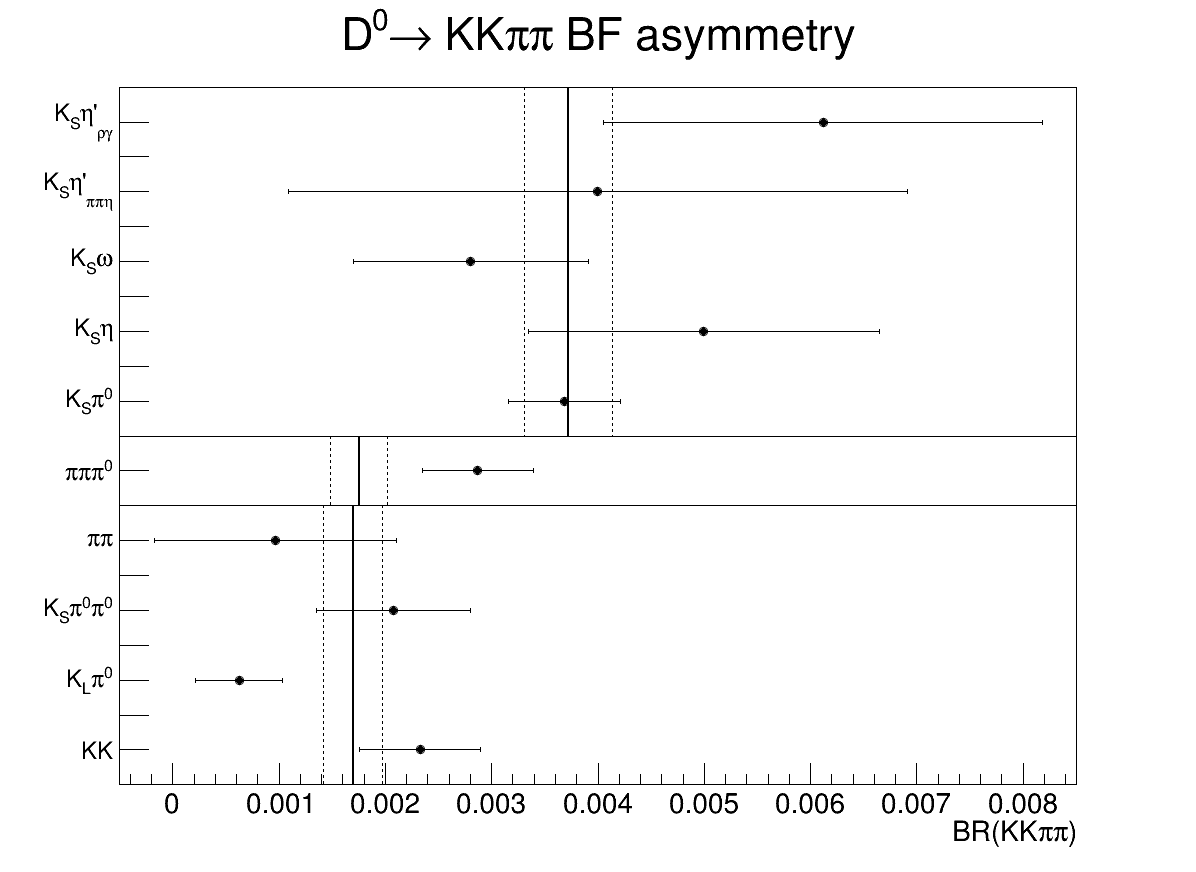
\includegraphics[width=0.75\textwidth]{Plots/CPeven_fraction_combination_CPtags.png}
    \caption{$F_+$ combination of CP tags\\Fit result: $F_+ = \SI{0.69(4)}{}$}
  \end{figure}
\end{frame}

\begin{frame}{$F_+$ measurement with $K_S\pi\pi$ tag}
  \begin{itemize}
    \item{With $K_S\pi\pi$, increase sensitivity through binning of $K_S\pi\pi$ phase space}
  \end{itemize}
  \begin{center}
    $M_j\propto\big(K^\prime_j + K^\prime_{-j} - 2\sqrt{K^\prime_jK^\prime_{-j}}c^\prime_j(2F_+^{KK\pi\pi - 1})\big)$
  \end{center}
  \begin{itemize}
    \item{Problem: $KK\pi\pi$ reconstruction efficiency is too low $\to$ Low yields!}
  \end{itemize}
  \begin{figure}
    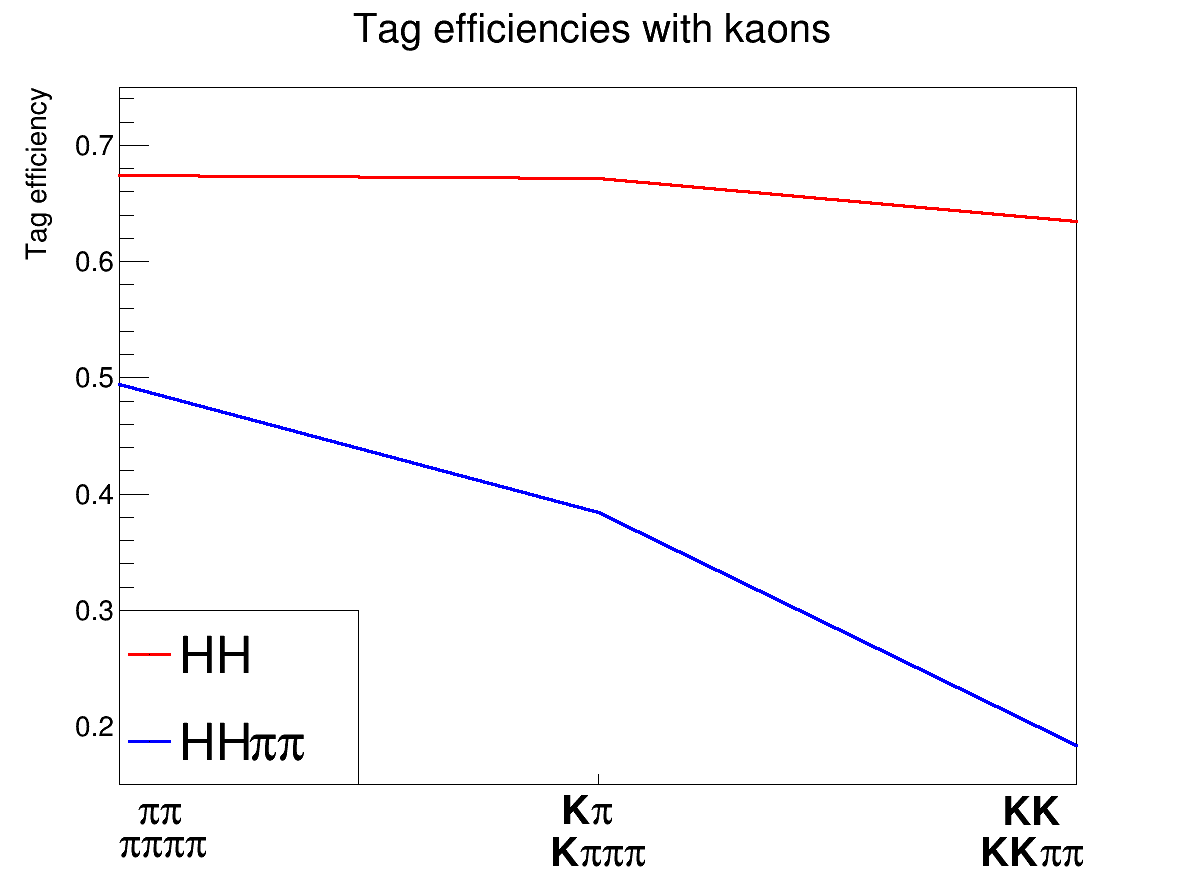
\includegraphics[width = 0.5\textwidth]{Plots/KaonTrackingEfficiency.png}
  \end{figure}
  \begin{itemize}
    \item{Likely explanation: Softer kaons $\to$ Kaons get stuck inside tracker}
  \end{itemize}
\end{frame}

\subsection{With \texorpdfstring{$K_{S, L}\pi\pi$}{K0pipi} tags}
\begin{frame}{$F_+$ measurement with $K_S\pi\pi$ tag}
  \begin{itemize}
    \setlength\itemsep{1.0em}
    \item{Solution: Partially reconstructed $KK\pi\pi$}
    \item{Strategy:}
    \begin{enumerate}
      \setlength\itemsep{0.5em}
      \item{Reconstruct $D\to K_S\pi\pi$}
      \item{Require 3 remaining good tracks consistent with $K\pi\pi$}
      \item{Use missing mass to reconstruct missing kaon}
    \end{enumerate}
  \end{itemize}
  \vspace{0.5cm}
  \def\arraystretch{1.2}%
  \begin{tabular}{l|c|c}
    Mode                                     & Inclusive yield & Double tag efficiency \\
    \hline
    $K_S\pi\pi$ (fully reconstructed)        & $67.2$          & $6.63 \pm 0.04$ \\
    $K_S\pi\pi$ (partially reconstructed)    & $85.9$          & $6.50 \pm 0.03$ \\
    $K_L\pi\pi$ (partially reconstructed)    & $176.9$         & $7.29 \pm 0.04$ \\
    \hline
  \end{tabular}
\end{frame}

\begin{frame}{Partially reconstructed $KK\pi\pi$ vs $K_S\pi\pi$}
  \begin{itemize}
    \item{Main challenge with partially reconstructed $KK\pi\pi$: $K\pi\pi\pi\pi^0$}
    \item{Require no $\pi^0$ candidates}
  \end{itemize}
  \begin{figure}
    \centering
    \vspace{-0.2cm}
    \begin{subfigure}{0.50\textwidth}
      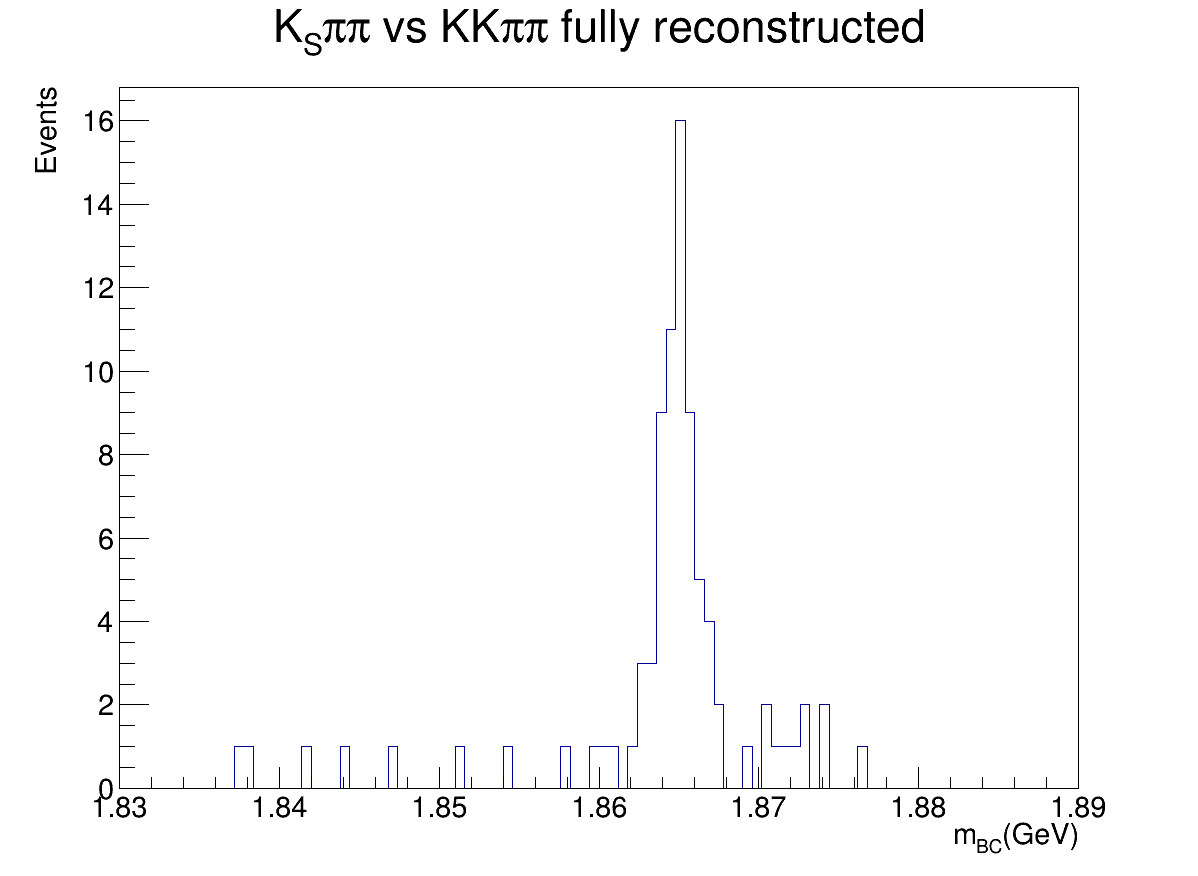
\includegraphics[width = 1.0\textwidth]{Plots/KKpipiVersusKSpipiMBC.png}
      \caption{Fully reconstructed}
    \end{subfigure}%
    \begin{subfigure}{0.50\textwidth}
      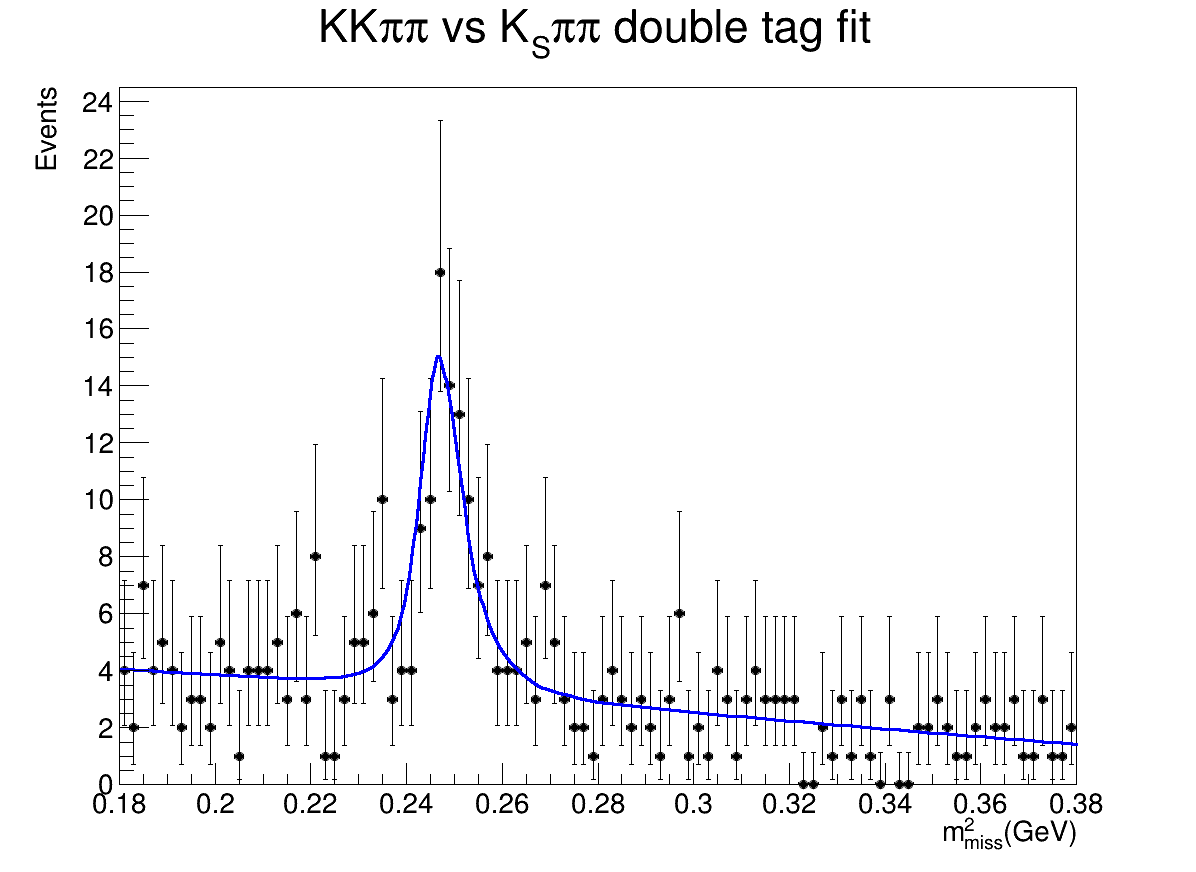
\includegraphics[width = 1.0\textwidth]{Plots/KSpipiPartReco_Inclusive_DoubleTagYield.png}
      \caption{Partially reconstructed}
    \end{subfigure}
    \caption{$KK\pi\pi$ vs $K_S\pi\pi$}
  \end{figure}
\end{frame}

\begin{frame}{Binned fit with $K_{S, L}\pi\pi$ tags}
  \begin{figure}
    \centering
    \vspace{-0.2cm}
    \begin{subfigure}{0.50\textwidth}
      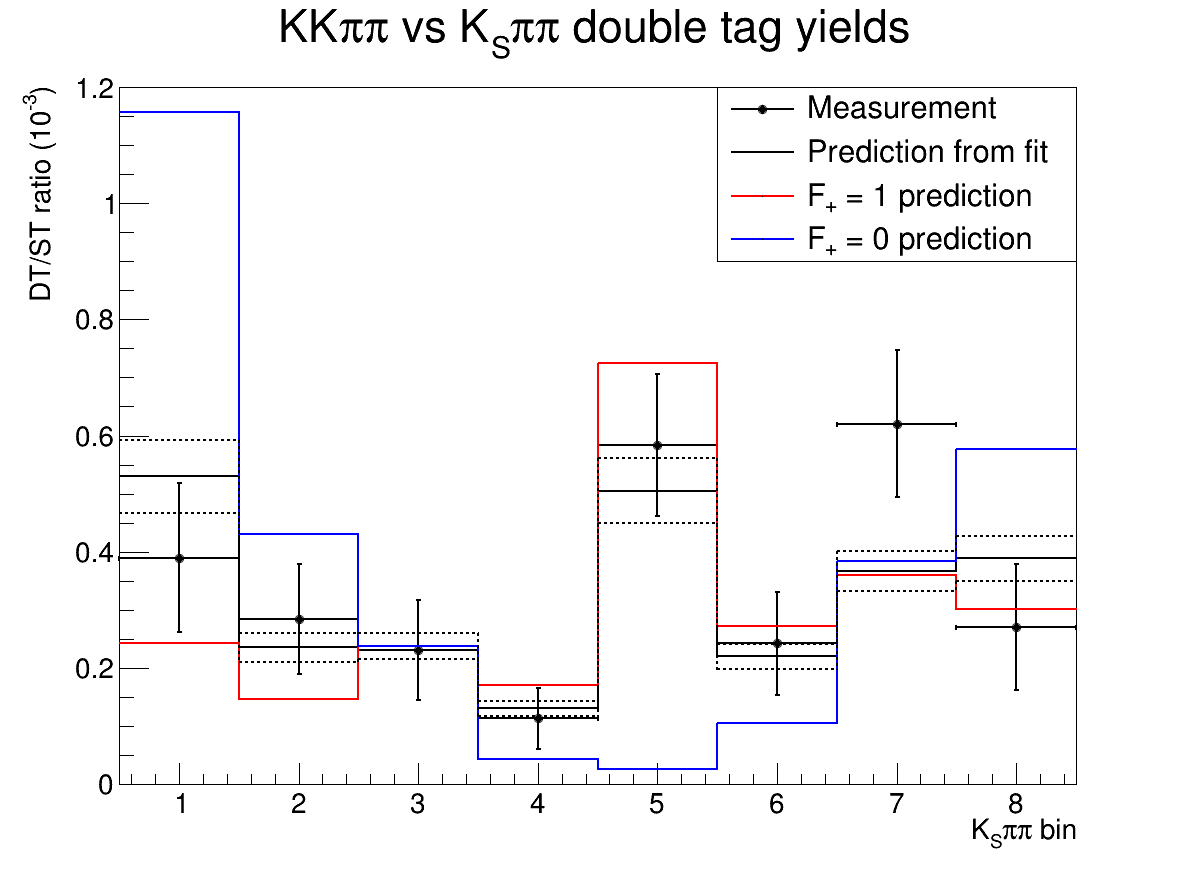
\includegraphics[width = 1.0\textwidth]{Plots/CPeven_fraction_combination_KSpipi.png}
      \caption{$K_S\pi\pi$\\Fit result: $F_+ = \SI{0.80(9)}{}$}
    \end{subfigure}%
    \begin{subfigure}{0.50\textwidth}
      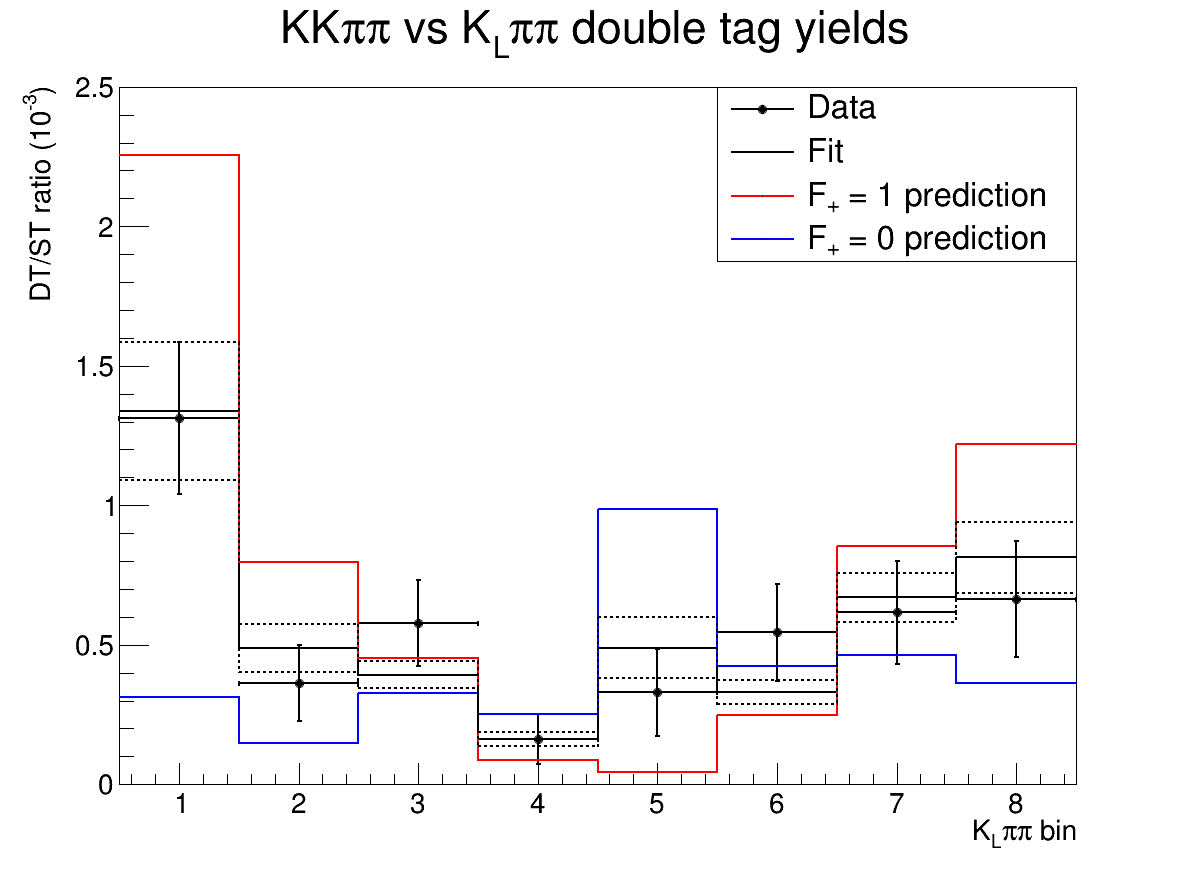
\includegraphics[width = 1.0\textwidth]{Plots/CPeven_fraction_combination_KLpipi.png}
      \caption{$K_L\pi\pi$\\Fit result: $F_+ = \SI{0.54(10)}{}$}
    \end{subfigure}
    \caption{$KK\pi\pi$ vs $K_{S, L}\pi\pi$ binned $F_+$ fit}
  \end{figure}
\end{frame}

\subsection{\texorpdfstring{$F_+$}{F+} combination}
\begin{frame}{$F_+$ combination}
  \begin{figure}
    \centering
    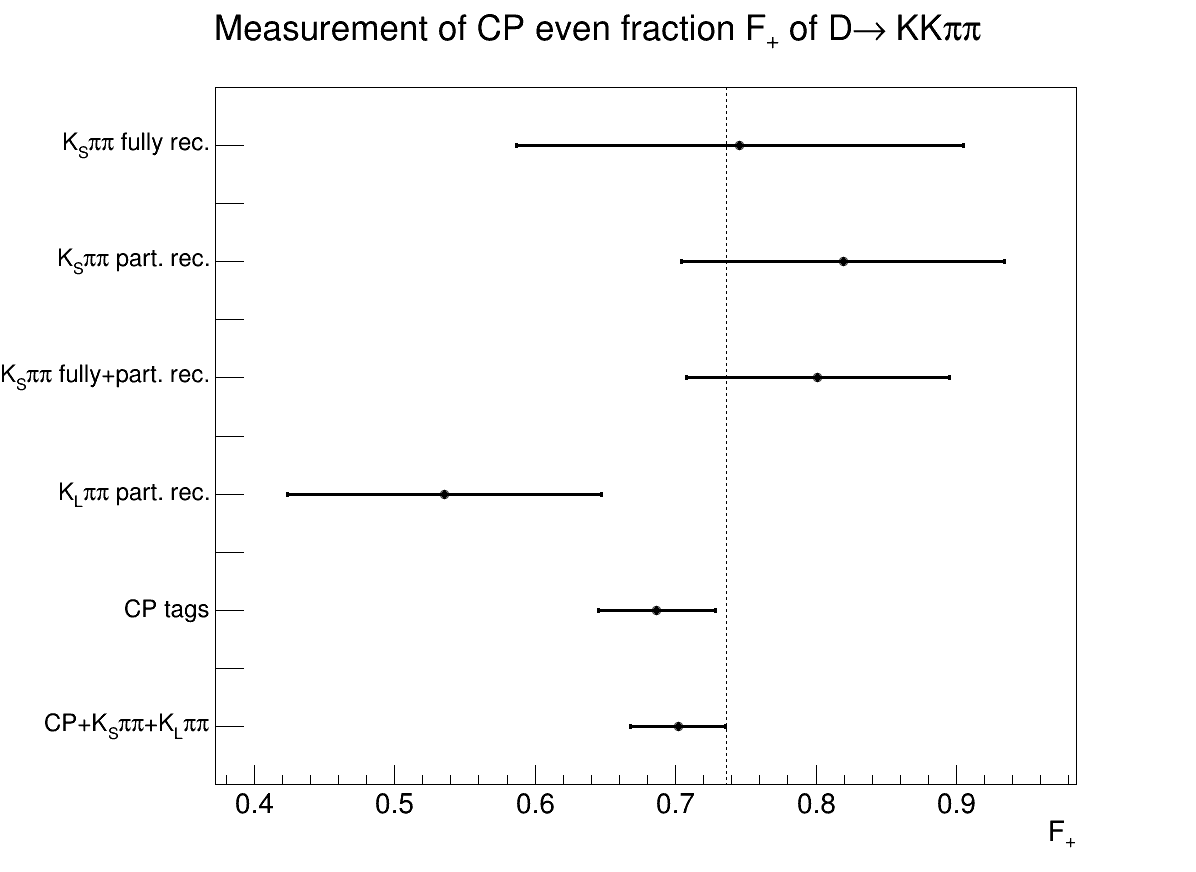
\includegraphics[width=0.75\textwidth]{Plots/FPlus_combination_comparison.png}
    \caption{Combination of $F_+$ measurements\\$F_+ = \SI{0.702(34)}{}$}
  \end{figure}
\end{frame}

\section{Summary and conclusion}

\begin{frame}{Summary}
  \begin{itemize}
    \setlength\itemsep{1.0em}
    \item{Good progress has been made on the strong-phase analysis of $D^0\to KK\pi\pi$}
    \begin{itemize}
      \item{$K_i$ is very consistent with LHCb model}
      \item{Expect sufficient statistics with $\SI{20}{\per\femto\barn}$ of $\psi(3770)$ data for a $c_i$/$s_i$ measurement with $2\times 8$ bins}
    \end{itemize}
    \item{$F_+$ has been measured using CP tags and $K_{S, L}\pi\pi$ tags}
    \begin{itemize}
      \item{Central value agrees with model}
      \item{Will allow all GLW analyses to include $KK\pi\pi$ to increase statistics}
    \end{itemize}
    \item{Next steps:}
    \begin{enumerate}
      \item{Finalise all peaking backgrounds}
      \item{Include partially reconstructed $KK\pi\pi$ vs $KK$, $\pi\pi\pi^0$ and $K_S\pi^0$}
      \item{Systematics studies}
      \item{Write up MEMO}
    \end{enumerate}
  \end{itemize}
  \begin{center}
    {\huge Thank you!}
  \end{center}
\end{frame}

\begin{frame}{Backup}
  \begin{center}
    {\huge Backup}
  \end{center}
\end{frame}

\begin{frame}{$K_S\omega$ CP even tag using sPlot}
  \begin{itemize}
    \setlength\itemsep{0.5em}
    \item{$D\to K_S\omega$ is CP odd}
    \item{CP-even contamination from non-resonant $D\to K_S\pi\pi\pi^0$}
    \begin{itemize}
      \item{$F_+(K_S\pi\pi\pi^0) = 0.238\pm0.012\pm0.012$ from CLEO}
    \end{itemize}
  \end{itemize}
  \begin{figure}
    \centering
    \vspace{-0.2cm}
    \begin{subfigure}{0.40\textwidth}
      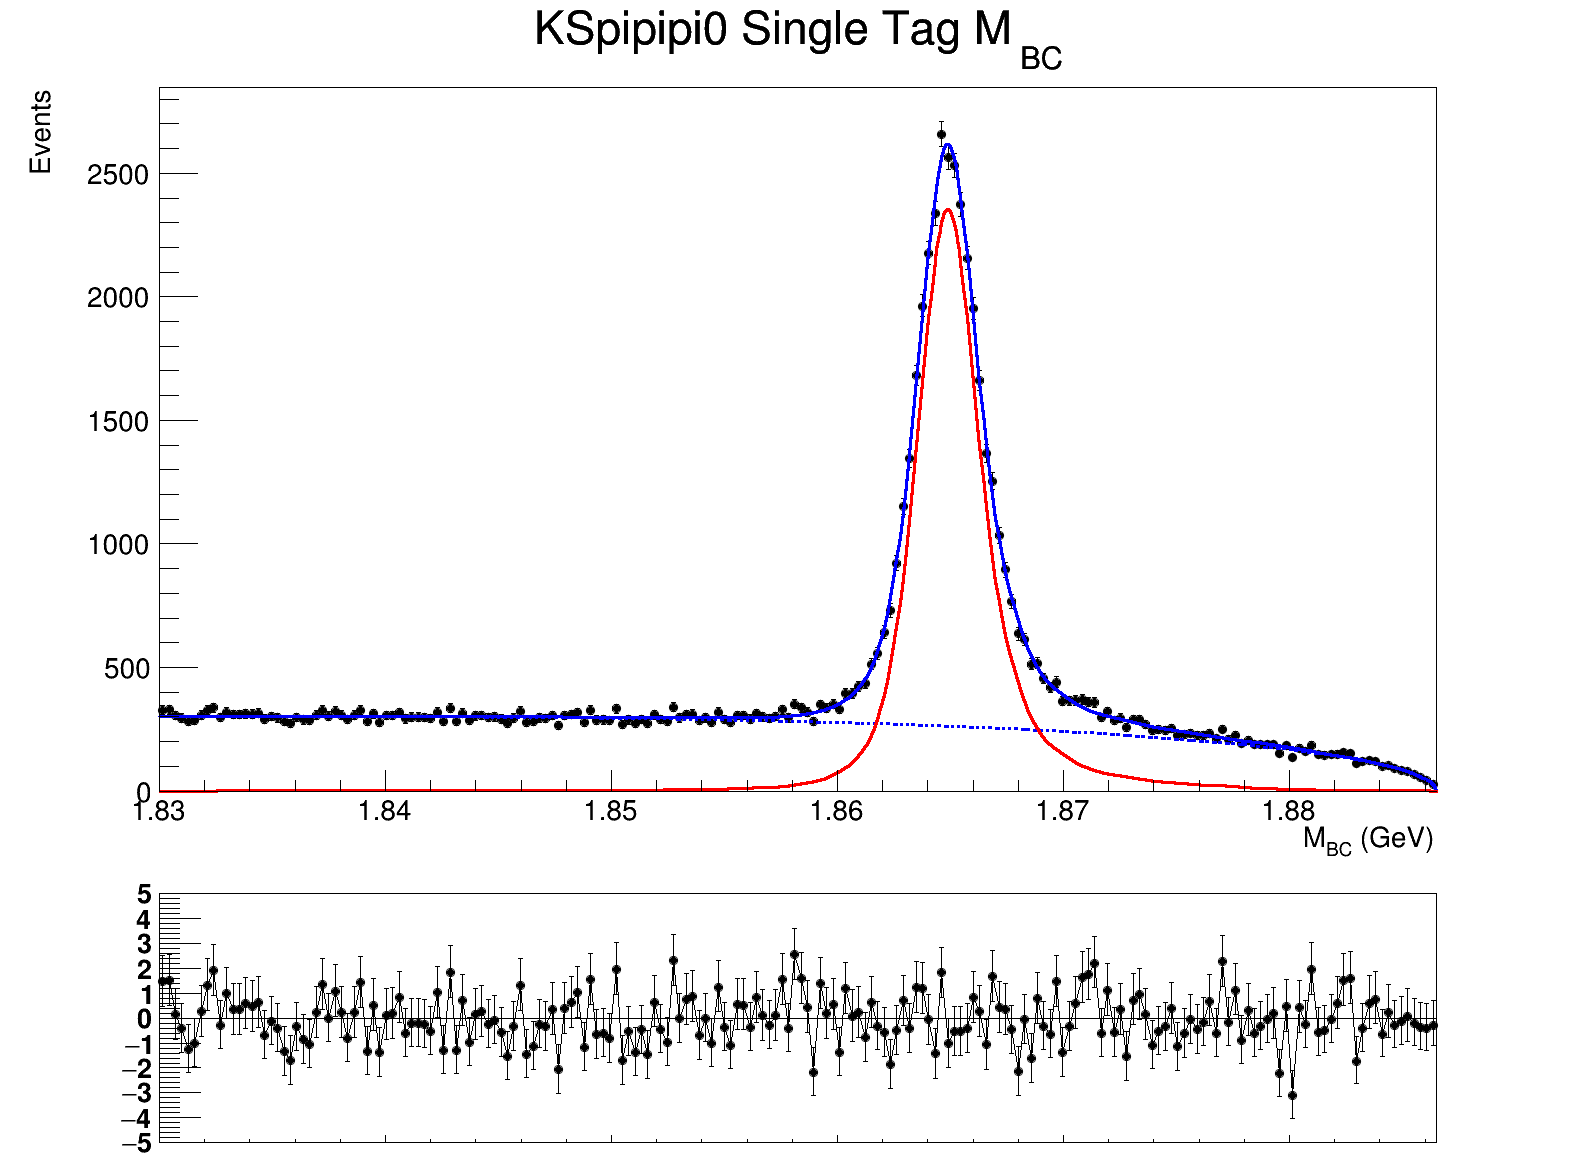
\includegraphics[width = 1.0\textwidth]{Plots/KSpipipi0_SingleTag_MBC_Plot.png}
      \caption{Single tag}
    \end{subfigure}%
    \begin{subfigure}{0.40\textwidth}
      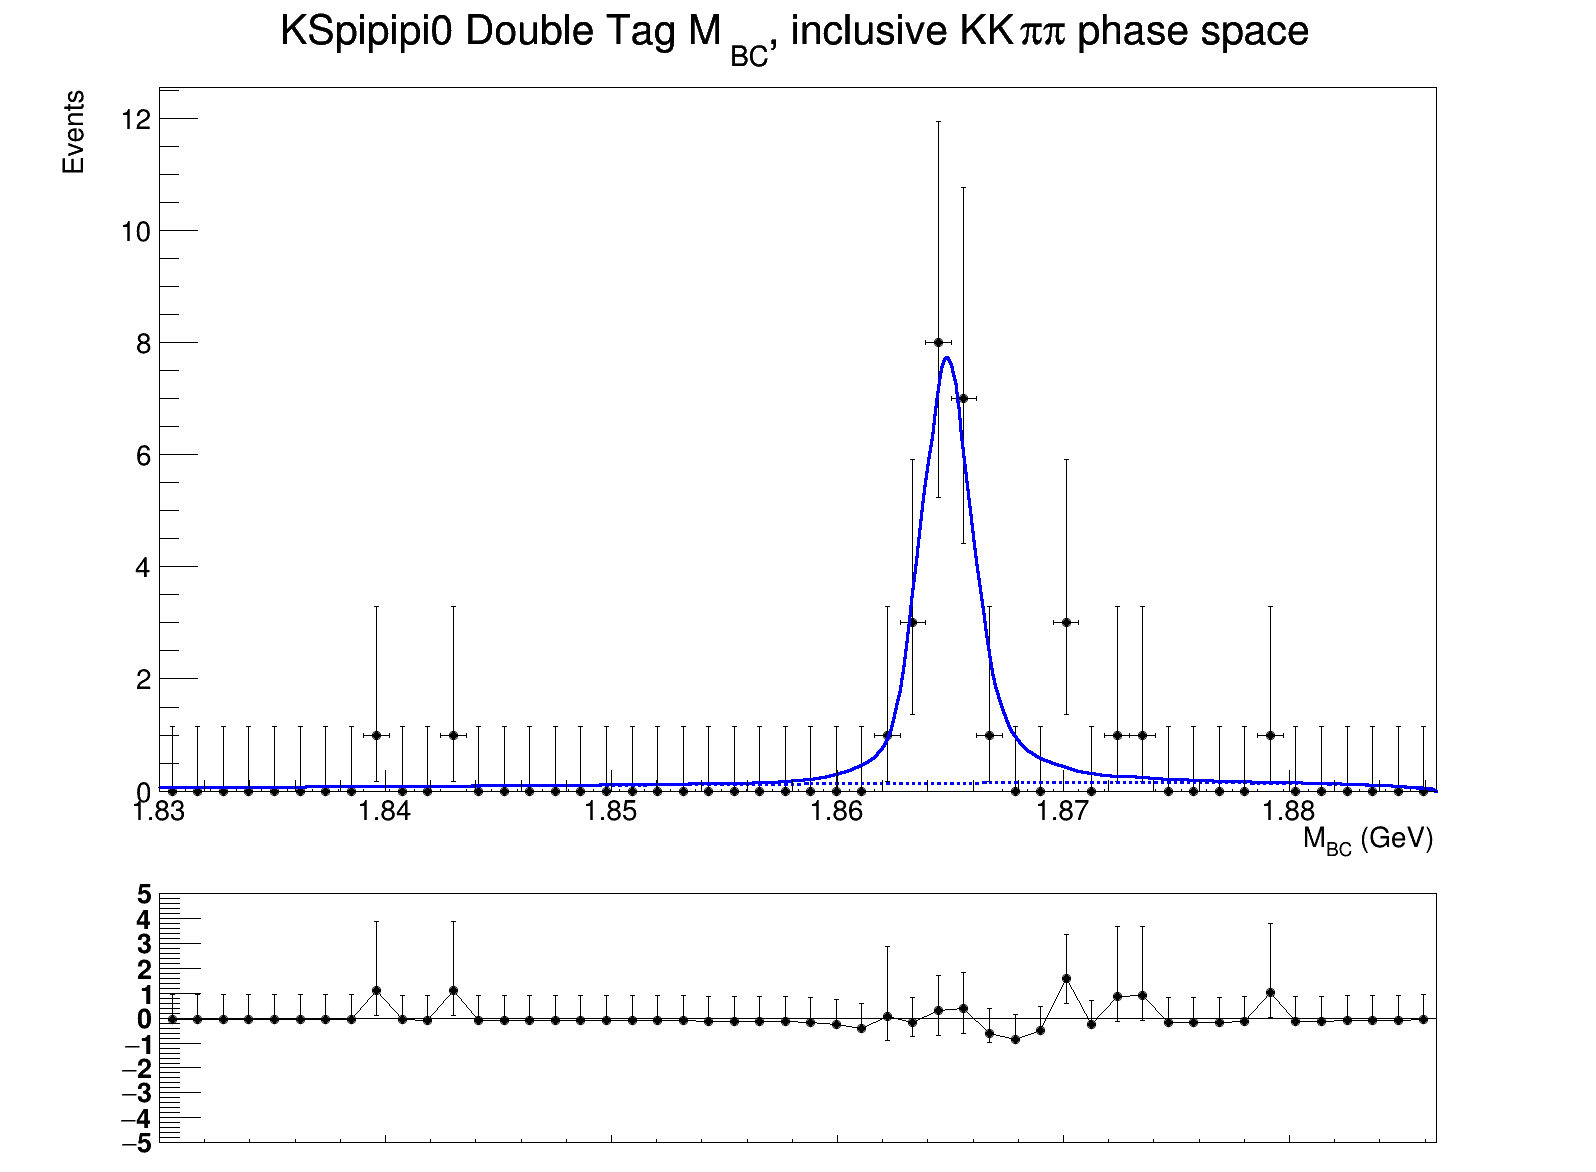
\includegraphics[width = 1.0\textwidth]{Plots/DoubleTagYield_DoubleTag_CP_KKpipi_vs_KSpipipi0_SignalBin0.png}
      \caption{Double tag}
    \end{subfigure}
    \caption{$D\to K_S\pi\pi\pi^0$ $D$ mass (beam constrained)}
  \end{figure}
\end{frame}

\begin{frame}{$K_S\omega$ CP even tag using sPlot}
  \begin{itemize}
    \item{Strategy:}
    \begin{enumerate}
      \item{From $D$ mass fit, remove non-$K_S\pi\pi\pi^0$ background using sPlot}
      \item{Fit $\pi\pi\pi^0$ invariant mass to obtain $K_S\omega$ yield}
    \end{enumerate}
  \end{itemize}
  \begin{figure}
    \centering
    \vspace{-0.2cm}
    \begin{subfigure}{0.40\textwidth}
      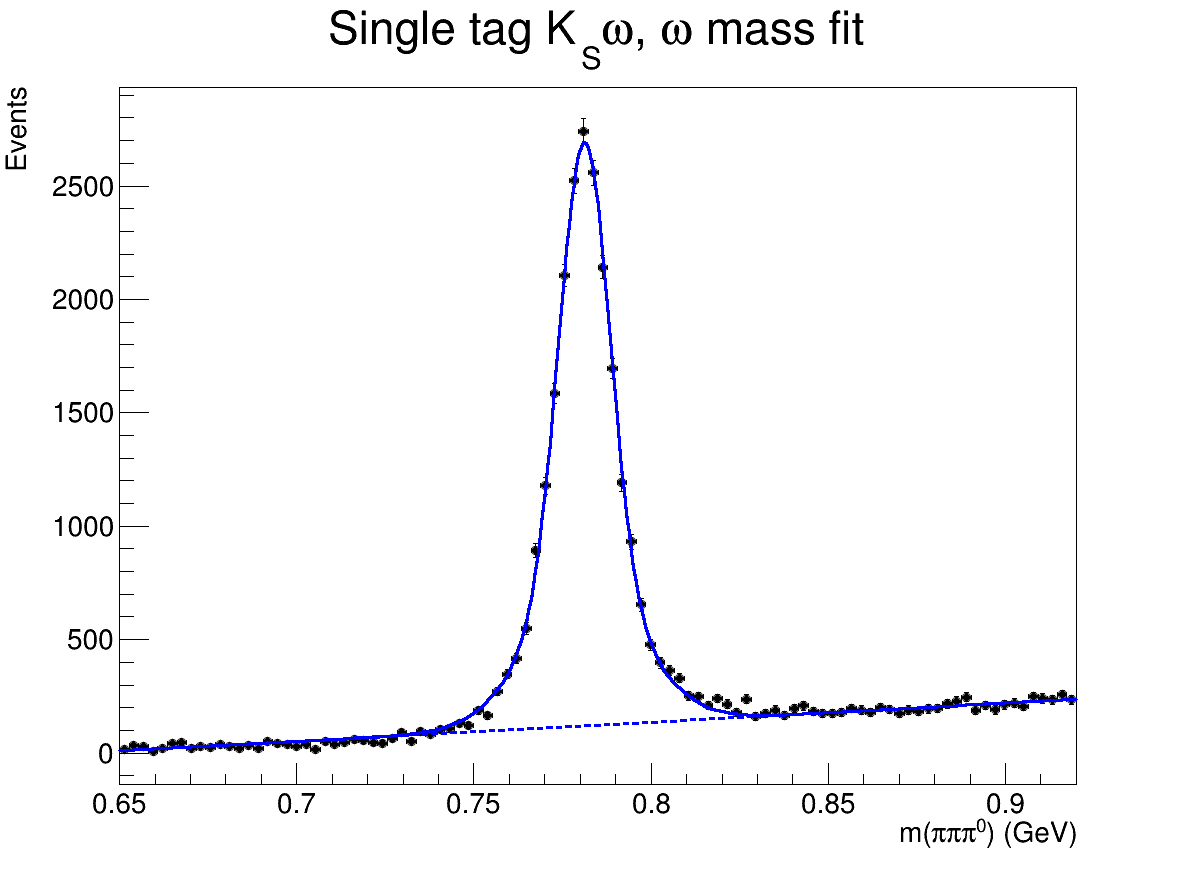
\includegraphics[width = 1.0\textwidth]{Plots/KSomega_ST_Mpipipi0.png}
      \caption{Single tag}
    \end{subfigure}%
    \begin{subfigure}{0.40\textwidth}
      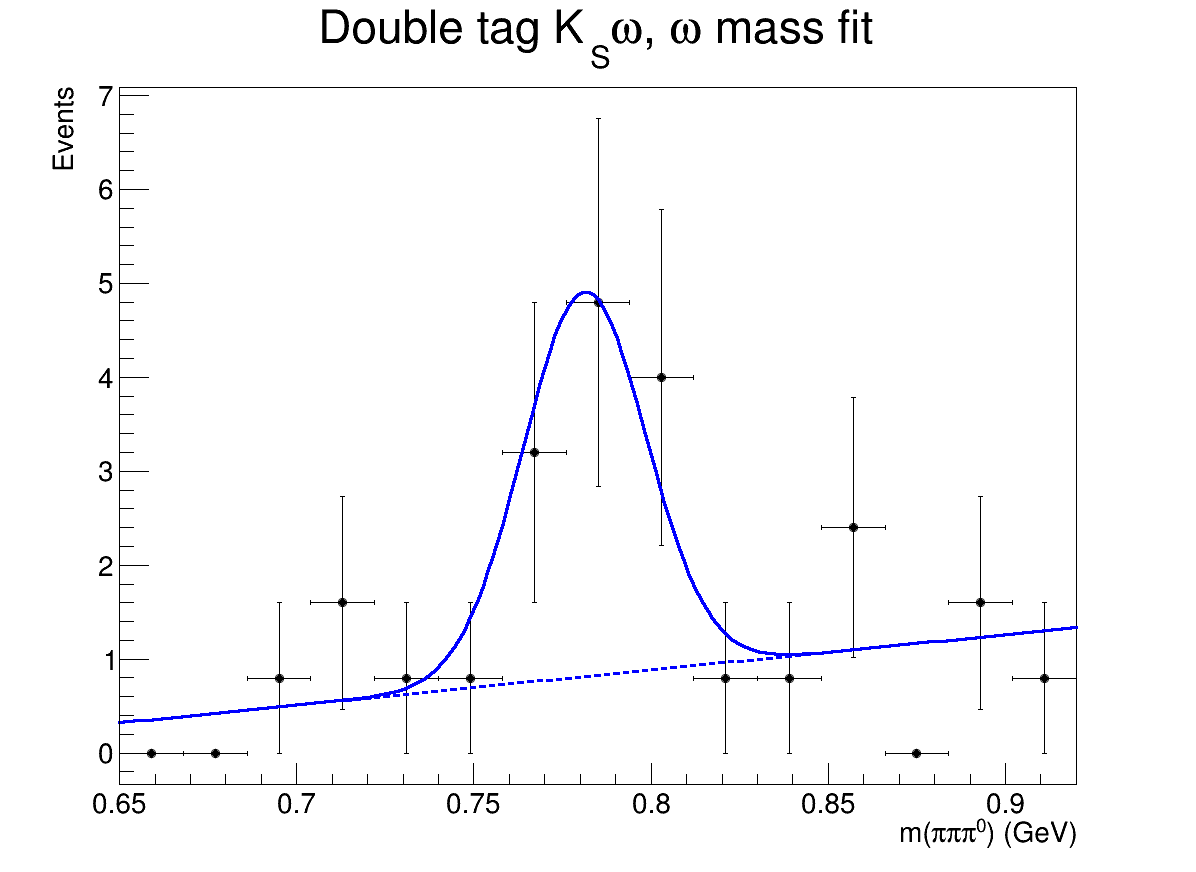
\includegraphics[width = 1.0\textwidth]{Plots/KSomega_DT_Mpipipi0.png}
      \caption{Double tag}
    \end{subfigure}
    \caption{$\pi\pi\pi^0$ invariant mass in $D\to K_S\pi\pi\pi^0$}
  \end{figure}
\end{frame}    

\end{document}
